\documentclass[aspectratio=169]{beamer}
\usetheme{vega}

\addbibresource{assets/pricing_lib.bib}

\usepackage{minted}
\newminted{python}{linenos=true,fontsize=\footnotesize}

\DeclareMathOperator*{\plim}{\ensuremath{\operatorname{\P-lim}}}

\newcommand{\cA}{\mathcal{A}}
\newcommand{\cB}{\mathcal{B}}
\newcommand{\cC}{\mathcal{C}}
\newcommand{\cN}{\mathcal{N}}

\subtitle{Student Research Group 'Stochastic Volatility Models', Project 'Heston--2'}
\title{Monte-Carlo Pricing under the Heston Model}
\author{Artemy Sazonov, Danil Legenky, Kirill Korban}
\institute{Lomonosov Moscow State Univesity, Faculty of Mechanics and Mathematics}
\date{February 25, 2023}

\begin{document}
    \maketitle

    \begin{frame}{Heston Model Definition}
        Assume that the spot asset at time $t$ follows the diffusion
        \begin{align}
            dS(t) & = \mu S(t)dt + \sqrt{v(t)} S(t) dZ_1(t), \label{Heston:price}\\
            dv(t) & = \kappa\left(\bar v -  v(t)\right) dt + \gamma\sqrt{v(t)} dZ_2(t), \label{Heston:variance}
        \end{align}
        where $Z_1$, $Z_2$ are the correlated Wiener processes with $dZ_1dZ_2 = \rho dt$.
    \end{frame}

    \section{Introduction to Monte-Carlo Methods}
        \subsection{Monte Carlo Simulation}
    \begin{frame}{Monte Carlo Simulation}{Statistical Estimation}
        \begin{lemma}
            Let $X_1, X_2, \dots, X_n$ be a series of independent and identically distributed random variables, and $h: \mathbb{R} \to \mathbb{R}$ be a borel function. Then $h(X_1), h(X_2), \dots, h(X_n)$ is a series of independent and identically distributed random variables.
        \end{lemma}
        Thus, we could write an unbiased consistent estimator of $\E \left[h(X)\right]$ as follows:
        \begin{equation}
            \widehat{\E \left[h(X)\right]} = \frac{1}{n} \sum_{i=1}^n h(X_i).
        \end{equation}
    \end{frame}

    \begin{frame}{Monte Carlo Simulation}{Local Truncation Error}
        \begin{definition}
            Monte Carlo simulation is a set of techniques that use pseudorandom number generators to solve problems that might be too complicated to be solved analytically. It is based on the central limit theorem.
        \end{definition}
        Asymptotic confidence interval for $\hat{\mu} = \widehat{\E\left[X\right]}$ at the confidence level $\alpha$:
        \begin{equation}
            \mu \in \left(\hat{\mu} - z_{\alpha/2} \sqrt{\frac{\sigma^2}{n}}, \hat{\mu} + z_{\alpha/2} \sqrt{\frac{\sigma^2}{n}}\right).
        \end{equation}
        That means that the estimation error is equal to $2z_{\alpha/2} \sqrt{\frac{\sigma^2}{n}}$.
    \end{frame}

    \begin{frame}{Discretization Schemes for SDEs}{Strong and weak convergence as a global truncation error analogue}
        \begin{definition}
            Let $\hat X^n(t)$ be a mesh approximation of an SDE solution $X(t)$ (we assume that there exists a unique strong solution). 
            Then a scheme is said to have a strong convergence of order $p$ if 
            \begin{equation}
                \E\left[\left|\hat X^n(T) - X(T)\right|\right] \leq Ch^p, \quad n \to \infty.
            \end{equation}
            A scheme is said to have a weak convergence of order $p$ if for any polynomial $f: \R \to \R$ we have
            \begin{equation}
                \left|\E\left[f(\hat X^n(T))\right] - \E\left[f(X(T))\right]\right| \leq Ch^p, \quad n \to \infty.
            \end{equation}
        \end{definition}
    \end{frame}

\subsection{Variance Reduction Methods}

    \begin{frame}{Variance Reduction Methods}{Control Variates}
        Suppose that we have another random variable $Z$ that is correlated with $Y$ and 
        $\E\left[Z\right] = \mu$ is known. Then we could introduce the following estimator:
        \begin{equation}
            \hat\theta^b = \bar Y + b(\bar Z - \mu),
        \end{equation}
        where $b$ is a constant. Obviously, $\hat\theta^b$ is a consistent unbiased estimator of 
        $\theta$. How do we choose $b$? We need to minimize the variance of $\hat\theta^b$. A simple 
        unconstrained optimization problem:
        \begin{equation*}
            \var \hat\theta^b = \var \bar Y + b^2 \var \bar Z - 2b \cov [\bar Y, \bar Z] \to \min_b.
        \end{equation*}
        The solution is
        \begin{equation}
            b^* = \frac{\cov [Y, Z]}{\var Z}.\label{eq:control_variates:bopt}
        \end{equation}
    \end{frame}

    \begin{frame}{Variance Reduction Methods}{Antithetic Variates}
        Suppose that we have two correlated identically distributed samples $Y^1$ and $Y^2$: $\cov[Y_i^1, Y_j^2] = \delta_{ij}\cov[Y_i^1, Y_i^2]$.
        Then we could introduce the following estimator:
        \begin{equation}
            \hat\theta_{\operatorname{AV}} = \frac{\bar Y^1 + \bar Y^2}{2}.
        \end{equation}
        Again, we can see that this estimator is unbiased and consistent. The variance of this estimator is
        \begin{equation*}
            \var \hat\theta_{\operatorname{AV}} = \frac{1}{4} \var[\bar Y^1] + \frac{1}{4} \var[\bar Y^2] + \frac{1}{2} \cov[\bar Y^1, \bar Y^2] .
        \end{equation*}
        Thus, the variance reduction effect takes place when $\rho < 0$. If $Y^1 = g(U)$, then its antithetic 
        variate is $Y^2 = g(1-U)$, where $U \sim U[0, 1]$. 
    \end{frame}

    \section{Discretization Methods}
        \begin{frame}{Euler Scheme for the Heston Model}{Modified Euler-Maruyama Discretization Scheme}
    Suppose we have the Heston model \eqref{Heston:price} -- \eqref{Heston:variance}. Then it could be numerically solved by the following finite difference scheme (for the log-prices $X(t)$):
    \begin{align}
        X_{n+1} & = X_n + (\mu - 0.5 v_n^+)h_n + \sqrt{v_n^+} \sqrt{h_n} Z_{1,n}, \label{Euler:Heston:price:posmod}\\
        v_{n+1} & = v_n + \left(\delta^2 - 2\beta v_n^+\right) h_n + \sigma \sqrt{v_n^+} \sqrt{h_n} Z_{2,n}, \label{Euler:Heston:variance:posmod}
    \end{align}
    and then we take the exponential of the log-prices:
    \begin{equation}
        S_{n} = S_0 e^{X_{n}}.
    \end{equation}
    
    However, the scheme is not accurate, since we ignore the $dZ_idZ_j$ terms in the It\^o-Taylor series approximation.
\end{frame}

\subsection{Quadratic-Exponential Discretization Scheme}
    \begin{frame}{Quadratic-Exponential Discretization Scheme}{Notation}\label{frame:Andersen:denotemeanstd}
        We denote 
        \begin{align}
            m    &= \E\left[\left.\hat{V}(t+\Delta)\right| \hat{V}(t)\right], \\
            s^2  &= \E\left[\left.\left(\hat{V}(t+\Delta) - m\right)^2\right| \hat{V}(t)\right], \\
            \psi &= \frac{s^2}{m^2}.
        \end{align}
    \end{frame}

    \begin{frame}{Quadratic-Exponential Discretization Scheme}{Idea}
        Andersen proposes an approximation based on moment-matching techniques. His goal is then to speed up the first step of Broadie and Kaya's method.
        He observes that the conditional distribution of $\hat{V}(t+\Delta)$ given $\hat{V}(t)$ visually difers when $\hat{V}(t)$ is small or large (in the variation coefficient sense).
        The scheme is constructed from the following two subschemes:
        \begin{enumerate}
            \item Quadratic sampling scheme ($\psi \leq 2$);
            \item Exponential sampling scheme ($\psi \geq 1$).
        \end{enumerate}
        Fortunately, these two intervals cover the whole positive real line. Furthermore, these two schemes could be applied at the same time when $\psi\in[1, 2]$. This implicates that there exist some critical value $\psi_{\text{crit}}\in[1, 2]$, which could be an indicator of which scheme is more applicable at the given value of $\psi$. Let us show you this.
    \end{frame}

    \begin{frame}{Quadratic-Exponential Discretization Scheme}{Quadratic case}
        For large enough $\hat{V}(t)$ we can approximate the distribution of $\hat{V}(t+\Delta)$ by the scaled non-central chi-squared distribution with $1$ degree of freedom:
        \begin{align}
            \law\left(\left.\hat{V}(t+\Delta) \right| \hat V(t)\right) =  a(\Delta, \hat{V}(t), VP) \chi'^2_1(b(\Delta, \hat{V}(t), VP)),
        \end{align}
        where $VP$ is the vector of parameters of the CIR variance.
        However, if $\hat{V}(t)$ is close to zero, then we have a problem in finding such $a = a(\Delta, \hat{V}(t), VP)$ and $b = b(\Delta, \hat{V}(t), VP)$ such that the moments of the desired conditional distribution could be properly matched.
    \end{frame}

    \begin{frame}{Quadratic-Exponential Discretization Scheme}{Exponential case}
        Therefore, we approximate the desired distribution with the following method. Let $\xi$ and $\eta$ be independent random variables and  $\xi \sim Be(1-p)$, $\eta \sim Exp(\beta)$ for some $p \in (0, 1)$ and $\beta > 0$. Then we have (given $\hat{V}(t)$)
        \begin{equation}
            \hat{V}(t+\Delta) = \xi\cdot\eta.
        \end{equation}
        Sampling $\xi$ and $\eta$: Smirnov's transform. Or we can use the Smirnov transform with the cdf of the desired distribution.
    \end{frame}

\subsection{Truncated Gaussian Discretization Scheme}
    \begin{frame}{Truncated Gaussian Discretization Scheme}{Idea}
        \begin{block}{Andersen:}
            \emph{In this scheme the idea is to sample from a moment-matched Gaussian density where all probability
            mass below zero is inserted into a delta-function at the origin.}
        \end{block} 
        Same, but in the formular form:
        \begin{equation}
            \left(\left.\hat{V}(t+\Delta)\right| V(t)\right) = \left(\mu + \sigma Z\right)^+,
        \end{equation}
        where $Z$ is a standard normal random variable and $\mu$ and $\sigma$ are the 'mean' and the 'standard deviation' of the desired distribution.
        We find $\mu$ and $\sigma$ from the same old moment-matching techniques (see Slide \ref{frame:Andersen:denotemeanstd}).
    \end{frame}

    \section{Practical Questions}
        \subsection{About Andersen's Article}
\subsection{Quadratic-Exponential Discretization Scheme}
    \begin{frame}{Quadratic-Exponential Discretization Scheme}{}\label{frame:Andersen:denotemeanstd}
        We denote 
        \begin{align}
            m    &= \E\left[\left.\hat{V}(t+\Delta)\right| \hat{V}(t)\right], \\
            s^2  &= \E\left[\left.\left(\hat{V}(t+\Delta) - m\right)^2\right| \hat{V}(t)\right], \\
            \psi &= \frac{s^2}{m^2}.
        \end{align}
    \end{frame}

    \begin{frame}{Quadratic-Exponential Discretization Scheme}{Idea}
        Andersen proposes an approximation based on moment-matching techniques. His goal is then to speed up the first step of Broadie and Kaya's method.
        He observes that the conditional distribution of $\hat{V}(t+\Delta)$ given $\hat{V}(t)$ visually difers when $\hat{V}(t)$ is small or large (in the variation coefficient sense).
        The scheme is constructed from the following two subschemes:
        \begin{enumerate}
            \item Quadratic sampling scheme ($\psi \leq 2$);
            \item Exponential sampling scheme ($\psi \geq 1$).
        \end{enumerate}
        Fortunately, these two intervals cover the whole positive real line. Furthermore, these two schemes could be applied at the same time when $\psi\in[1, 2]$. This implicates that there exist some critical value $\psi_{\text{crit}}\in[1, 2]$, which could be an indicator of which scheme is more applicable at the given value of $\psi$. Let us show you this.
    \end{frame}

    \begin{frame}{Quadratic-Exponential Discretization Scheme}{Quadratic case}
        For large enough $\hat{V}(t)$ we can approximate the distribution of $\hat{V}(t+\Delta)$ by the scaled non-central chi-squared distribution with $1$ degree of freedom:
        \begin{align}
            \law\left(\left.\hat{V}(t+\Delta) \right| \hat V(t)\right) =  a(\Delta, \hat{V}(t), VP) \chi'^2_1(b(\Delta, \hat{V}(t), VP)),
        \end{align}
        where $VP$ is the vector of parameters of the CIR variance.
        However, if $\hat{V}(t)$ is close to zero, then we have a problem in finding such $a = a(\Delta, \hat{V}(t), VP)$ and $b = b(\Delta, \hat{V}(t), VP)$ such that the moments of the desired conditional distribution could be properly matched.
    \end{frame}

    \begin{frame}{Quadratic-Exponential Discretization Scheme}{Exponential case}
        Therefore, we approximate the desired distribution with the following method. Let $\xi$ and $\eta$ be independent random variables and  $\xi \sim Be(1-p)$, $\eta \sim Exp(\beta)$ for some $p \in (0, 1)$ and $\beta > 0$. Then we have (given $\hat{V}(t)$)
        \begin{equation}
            \hat{V}(t+\Delta) = \xi\cdot\eta.
        \end{equation}
        Sampling $\xi$ and $\eta$: Smirnov's transform. Or we can use the Smirnov transform with the cdf of the desired distribution.
    \end{frame}

\subsection{Truncated Gaussian Discretization Scheme}
    \begin{frame}{Truncated Gaussian Discretization Scheme}{Idea}
        \begin{block}{Andersen:}
            \emph{In this scheme the idea is to sample from a moment-matched Gaussian density where all probability
            mass below zero is inserted into a delta-function at the origin.}
        \end{block} 
        Same, but in the formular form:
        \begin{equation}
            \left(\left.\hat{V}(t+\Delta)\right| V(t)\right) = \left(\mu + \sigma Z\right)^+,
        \end{equation}
        where $Z$ is a standard normal random variable and $\mu$ and $\sigma$ are the 'mean' and the 'standard deviation' of the desired distribution.
        We find $\mu$ and $\sigma$ from the same old moment-matching techniques (see Slide \ref{frame:Andersen:denotemeanstd}).
    \end{frame}

    \section{Accuracy-Performance Trade-Off Analysis}
        \begin{frame}{The Surface of Errors}{Params \#3: $\kappa = 0.5$, $\gamma = 1$, $\rho = -0.9$, $\bar v = 0.04$, $v_0 = 0.04$}
    \begin{figure}
        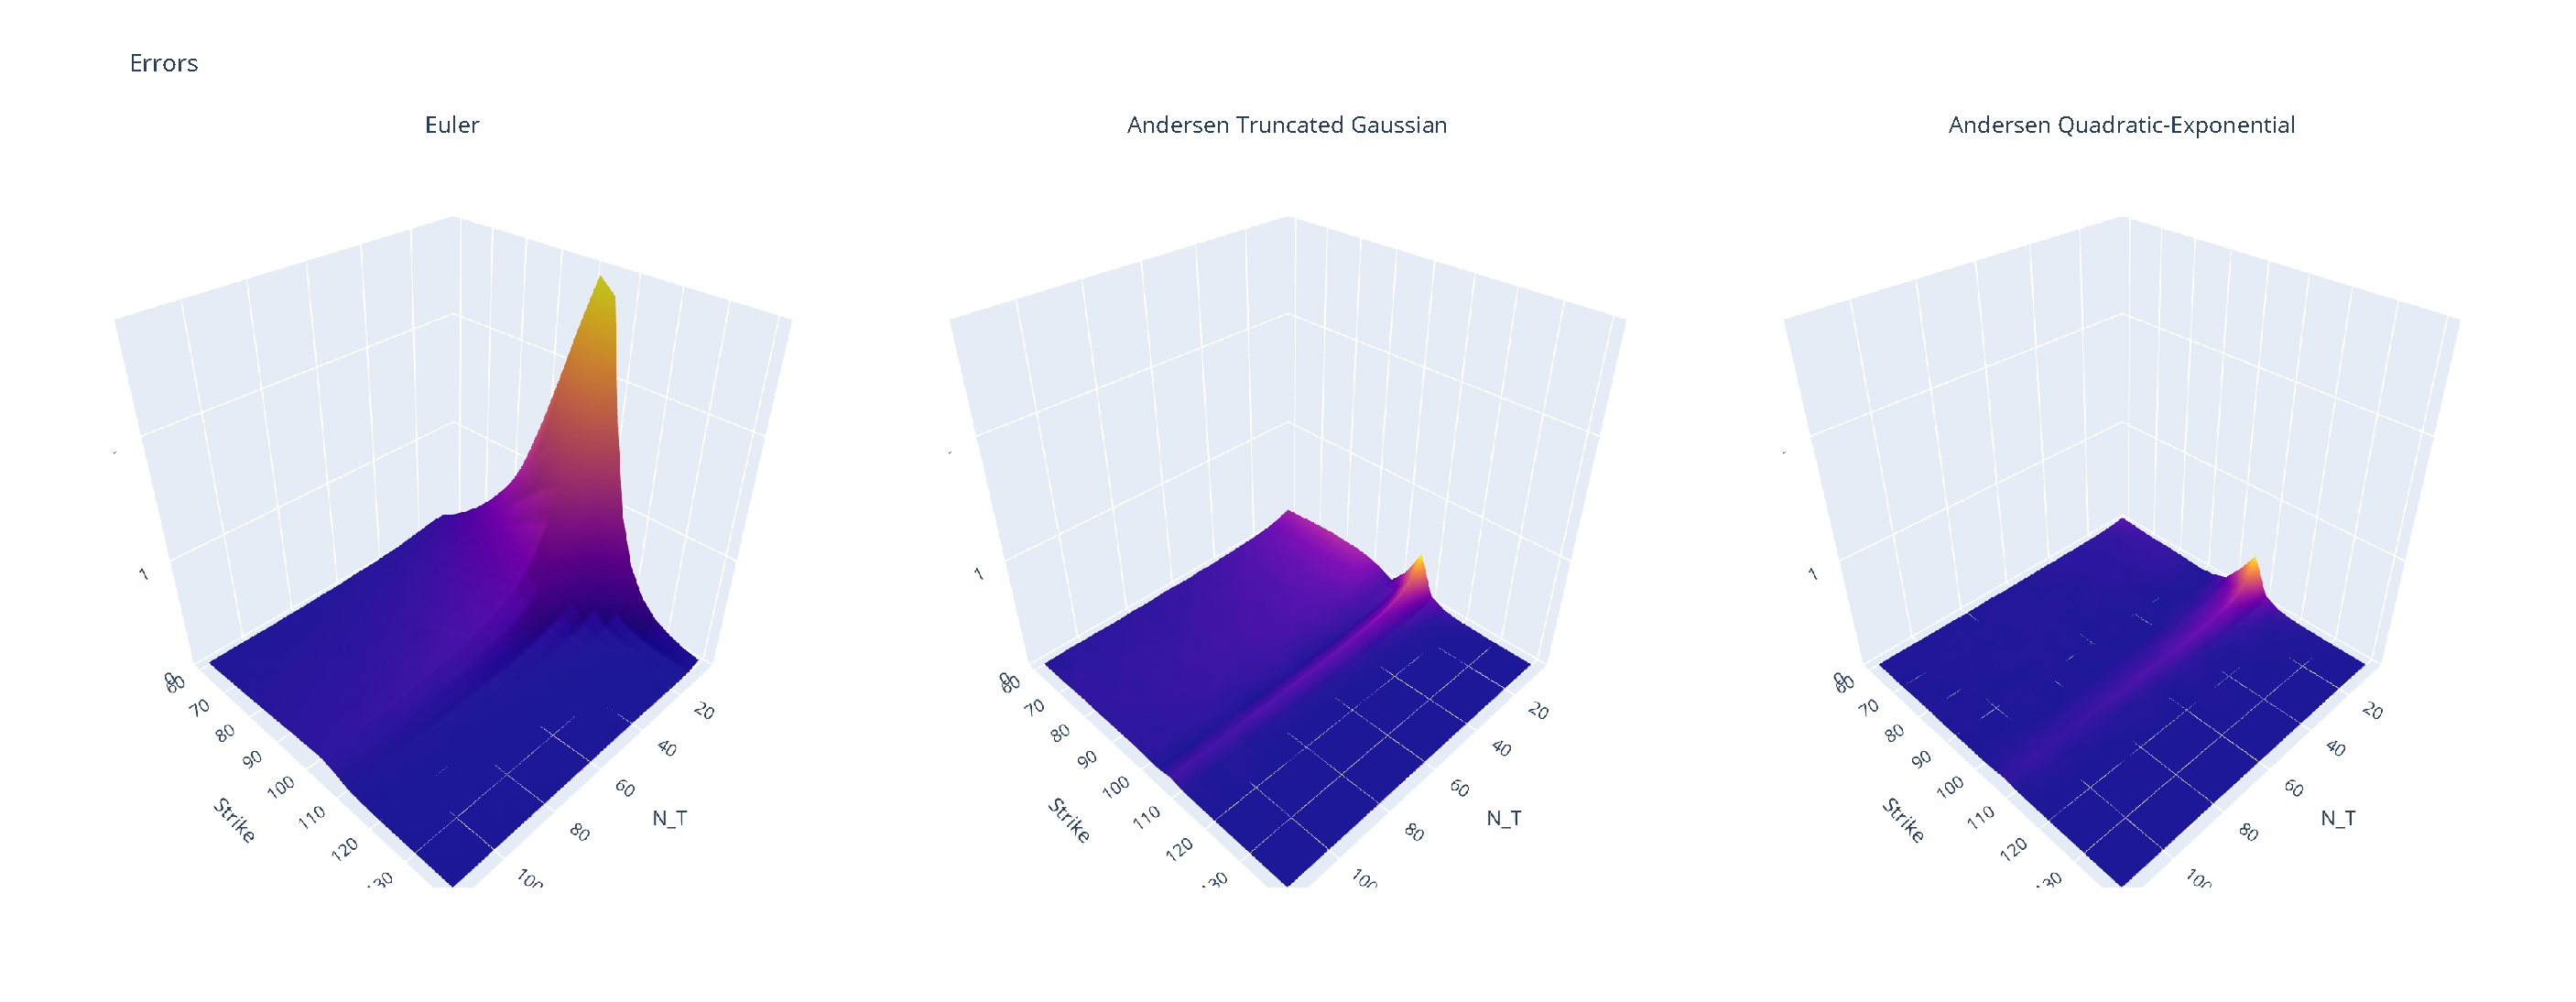
\includegraphics[width=\textwidth]{part4/pictures/err_surface_strike_N_T.pdf}
        \caption{$T=1$, \texttt{absolute\_error = 1e-2}}
    \end{figure}
\end{frame}

\begin{frame}{The Surface of Errors}{Params \#1: $\kappa = 1.3125$, $\gamma = 0.5125$, $\rho = -0.3937$, $\bar v = 0.0641$, $v_0 = 0.3$}
    \begin{figure}
        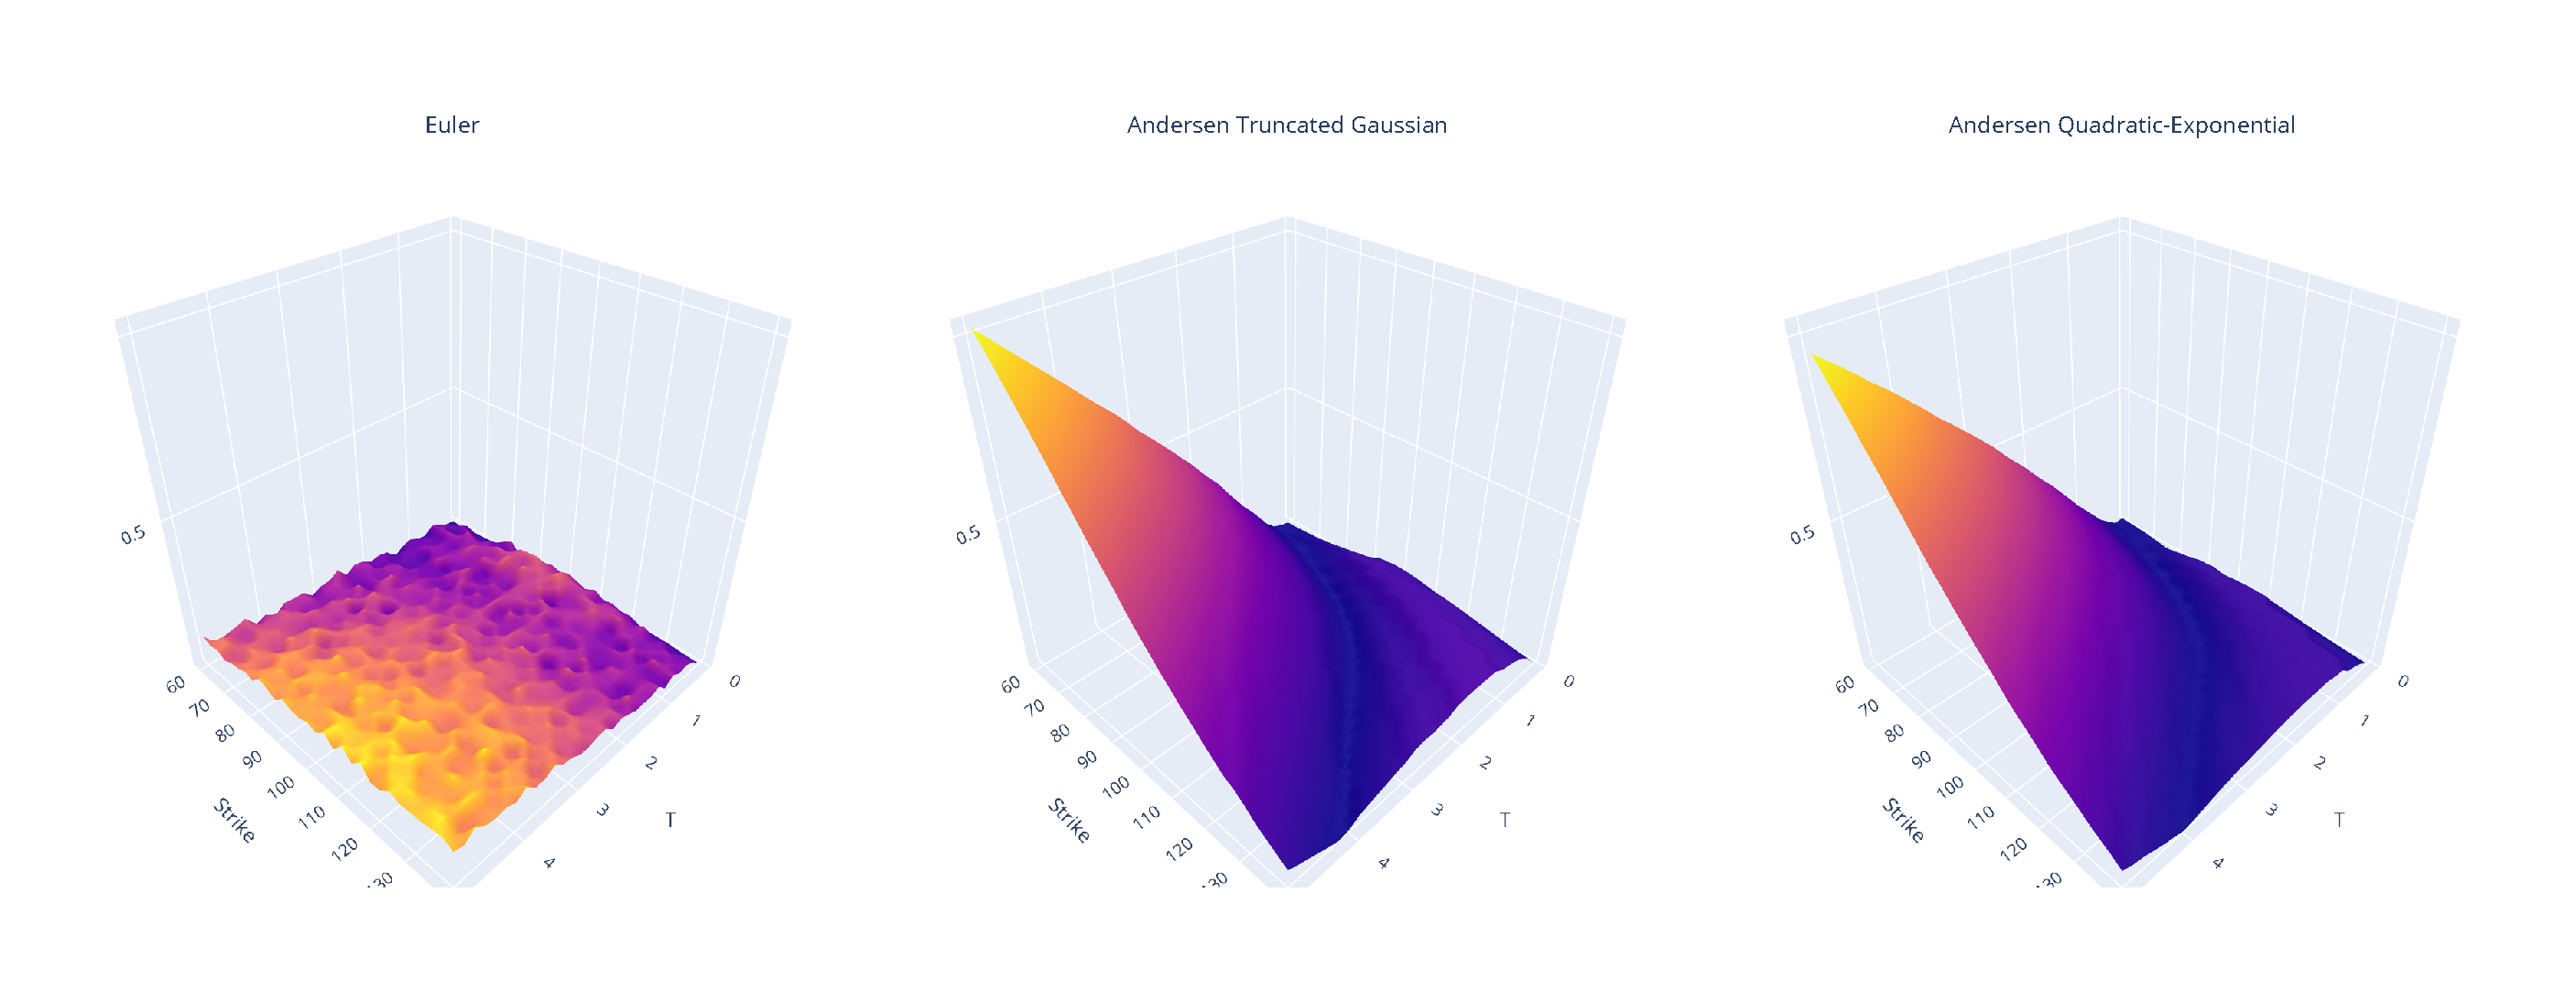
\includegraphics[width=\textwidth]{part4/pictures/err_surface_strike_T_N_T=50_param1.pdf}
        \caption{\texttt{N\_T = 50}, \texttt{absolute\_error = 1e-2}}
    \end{figure}
\end{frame}

\begin{frame}{The Surface of Errors}{Params \#2: $\kappa = 1$, $\gamma = 0.4$, $\rho = -0.1$, $\bar v = 0.2$, $v_0 = 0.2$}
    \begin{figure}
        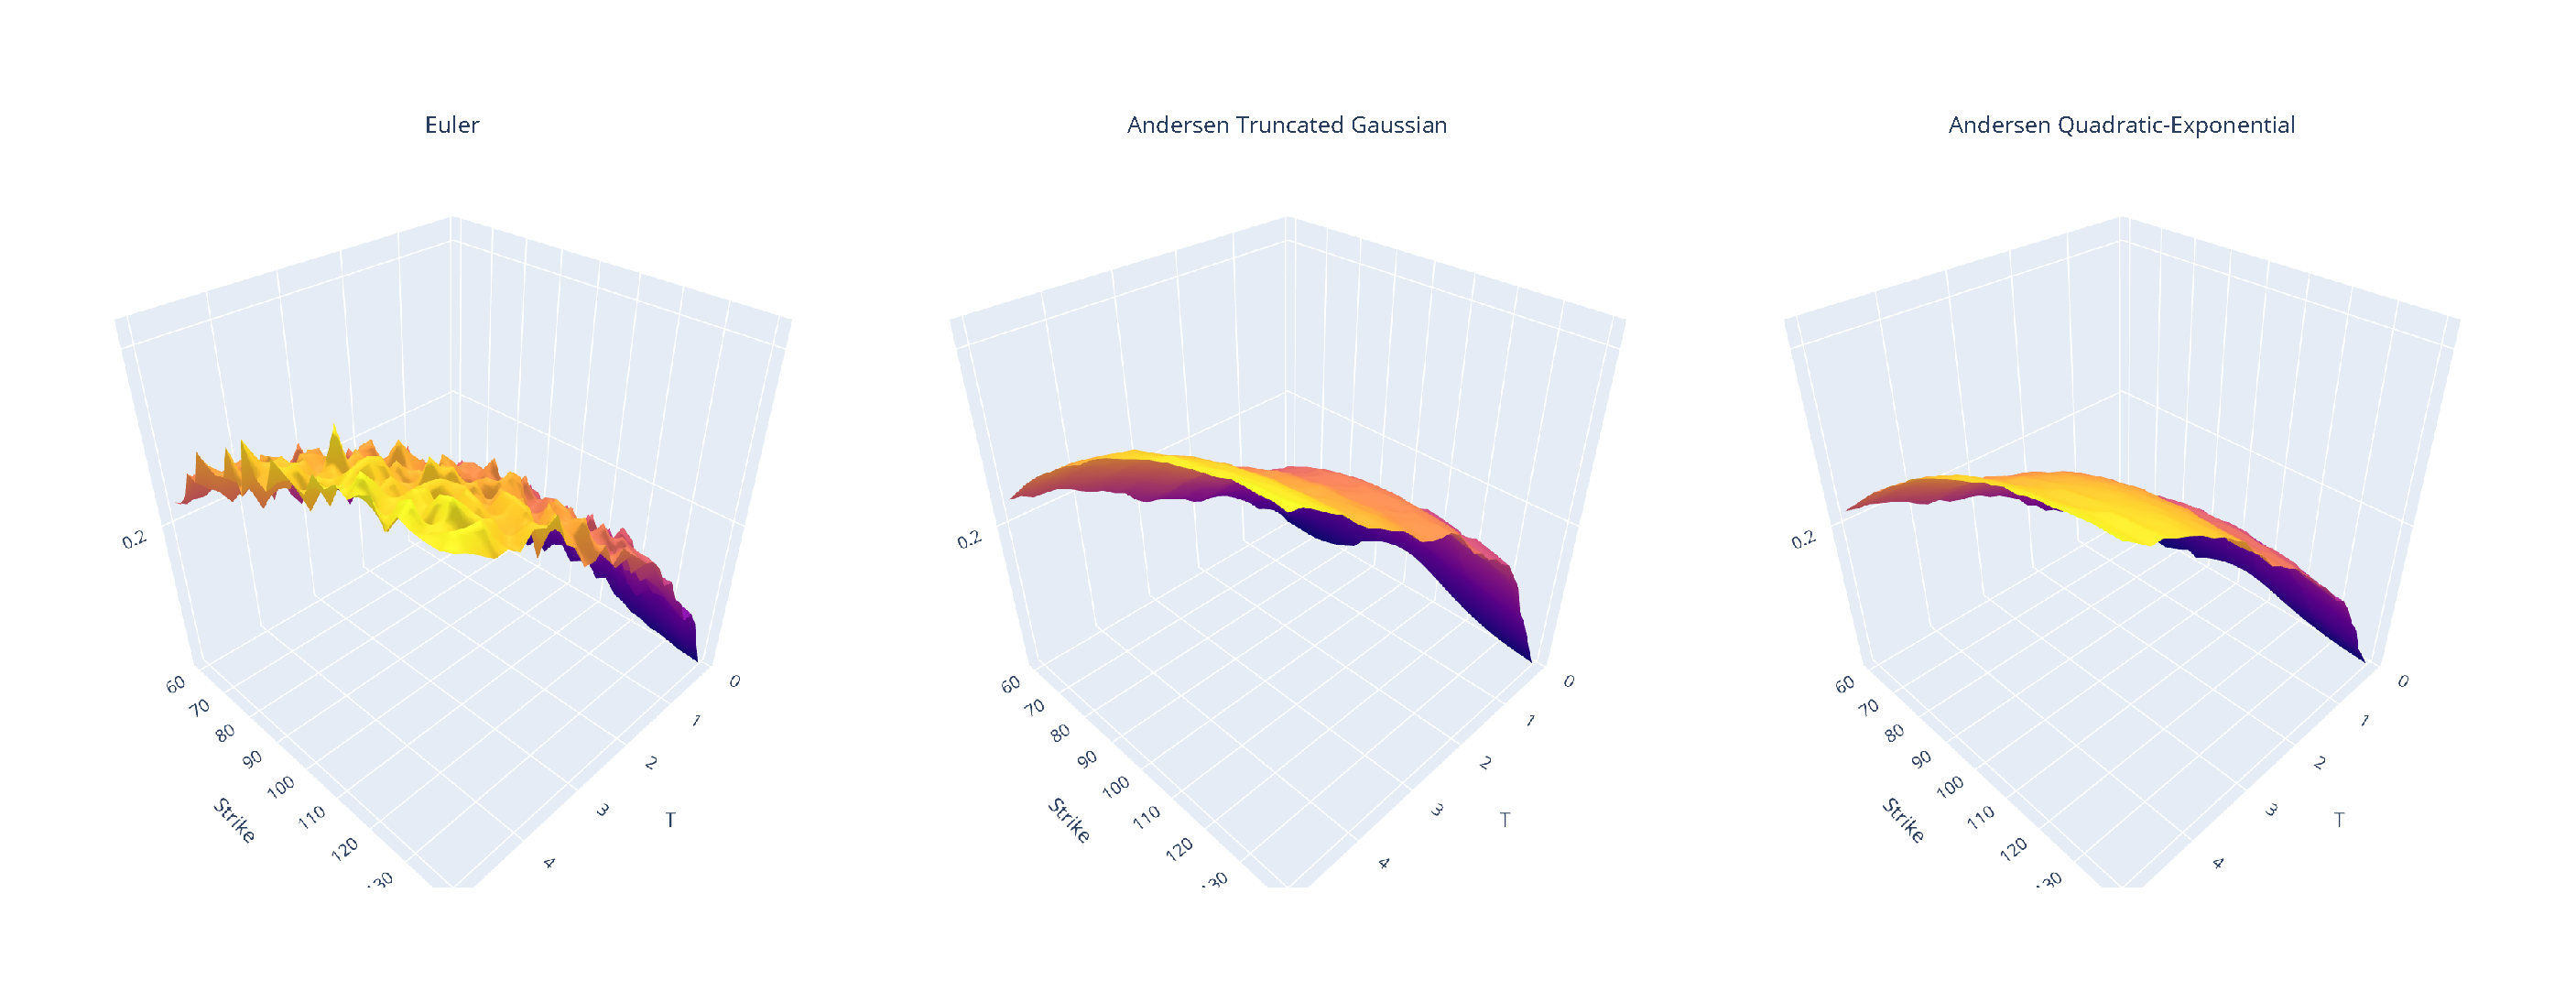
\includegraphics[width=\textwidth]{part4/pictures/err_surface_strike_T_N_T=50_param2.pdf}
        \caption{\texttt{N\_T = 50}, \texttt{absolute\_error = 1e-2}}
    \end{figure}
\end{frame}

\begin{frame}{The Surface of Errors}{Params \#3: $\kappa = 0.5$, $\gamma = 1$, $\rho = -0.9$, $\bar v = 0.04$, $v_0 = 0.04$}
    \begin{figure}
        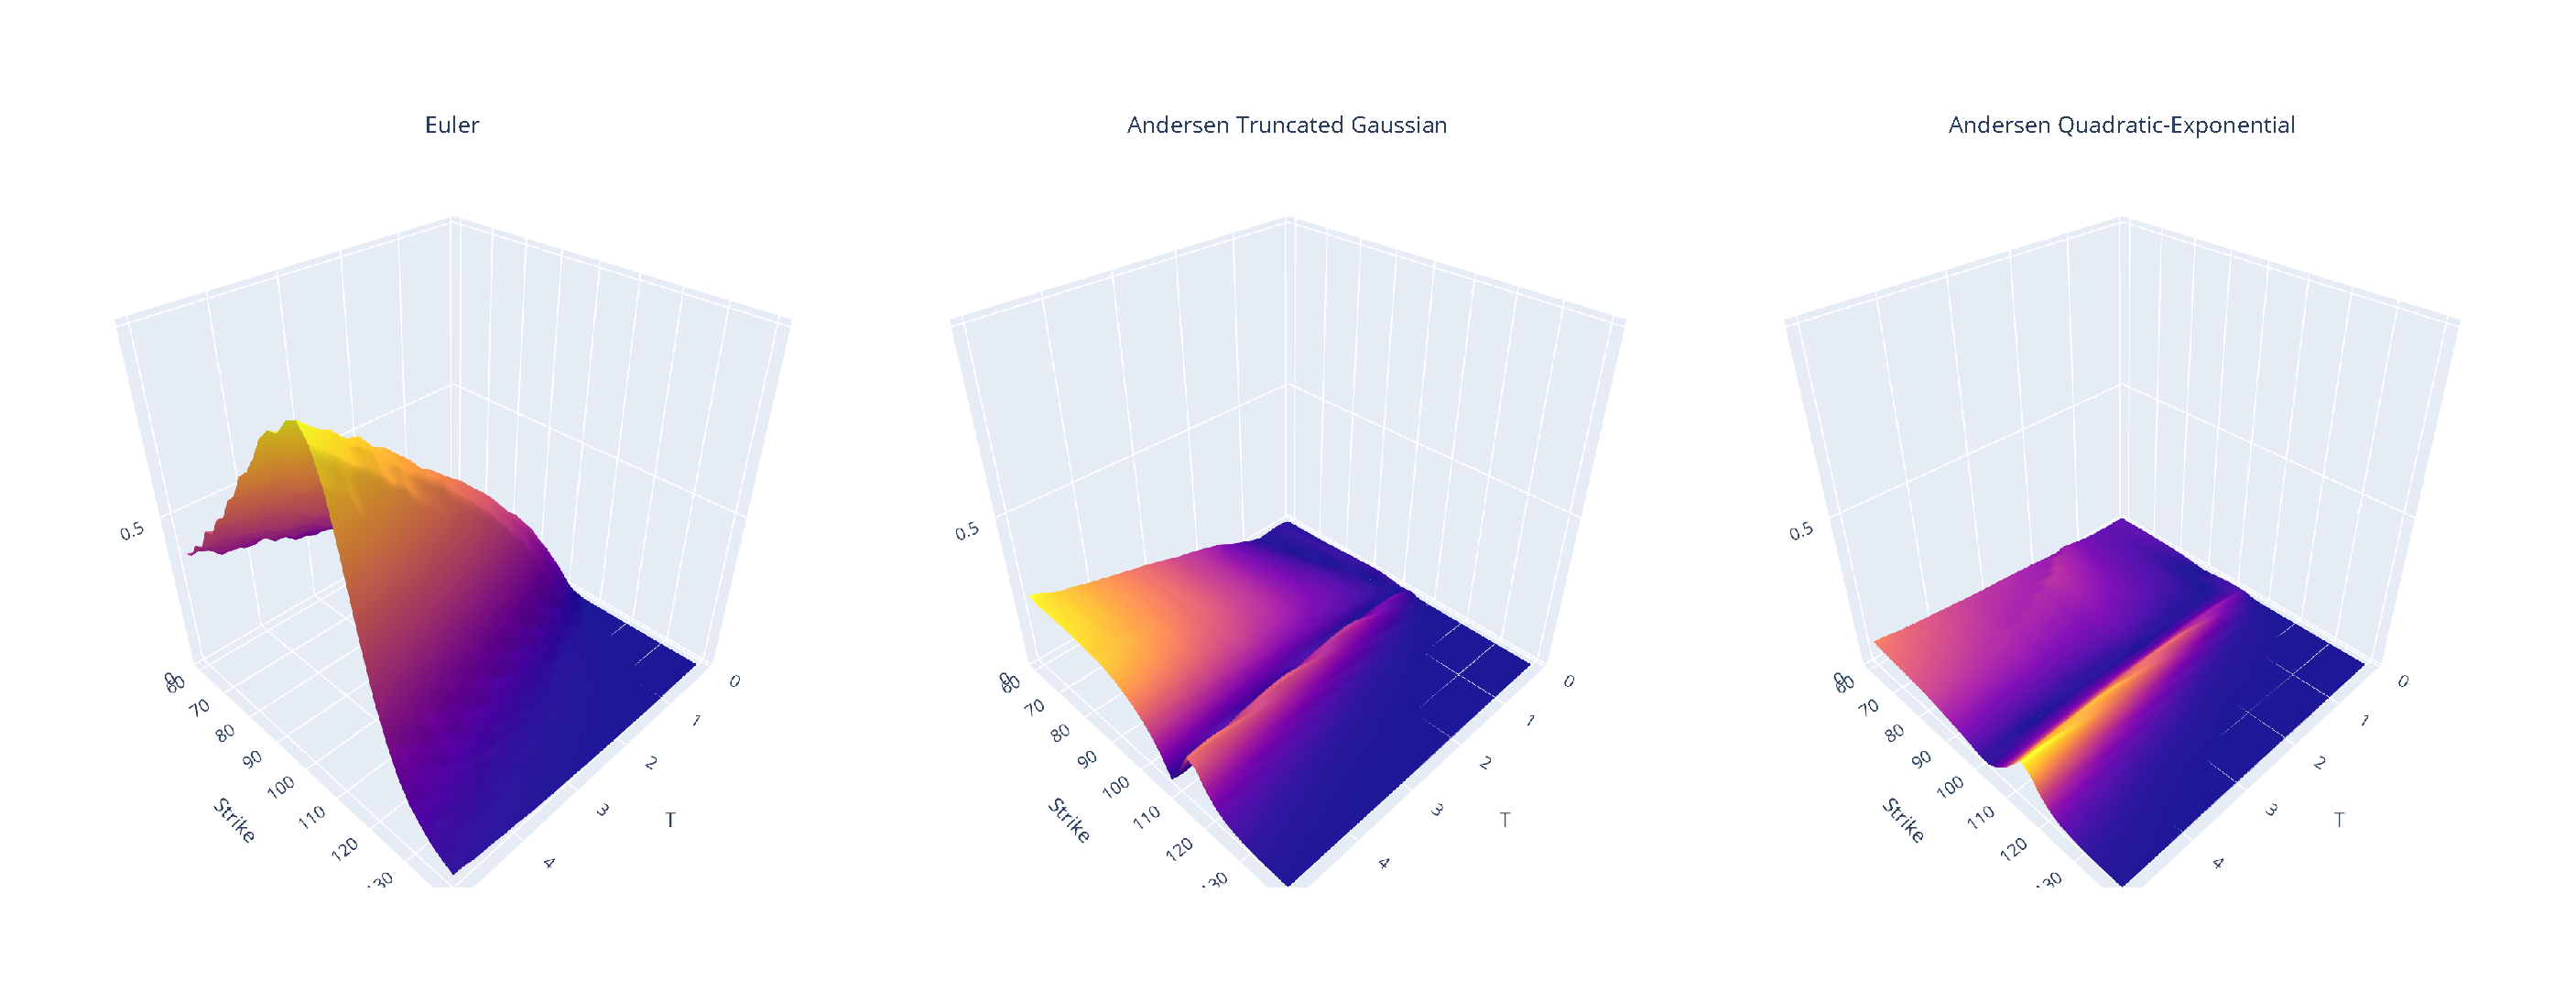
\includegraphics[width=\textwidth]{part4/pictures/err_surface_strike_T_N_T=50_param3.pdf}
        \caption{\texttt{N\_T = 50}, \texttt{absolute\_error = 1e-2}}
    \end{figure}
\end{frame}

\begin{frame}{The Surface of Errors}{Params \#4: $\kappa = 0.3$, $\gamma = 0.9$, $\rho = -0.5$, $\bar v = 0.04$, $v_0 = 0.04$}
    \begin{figure}
        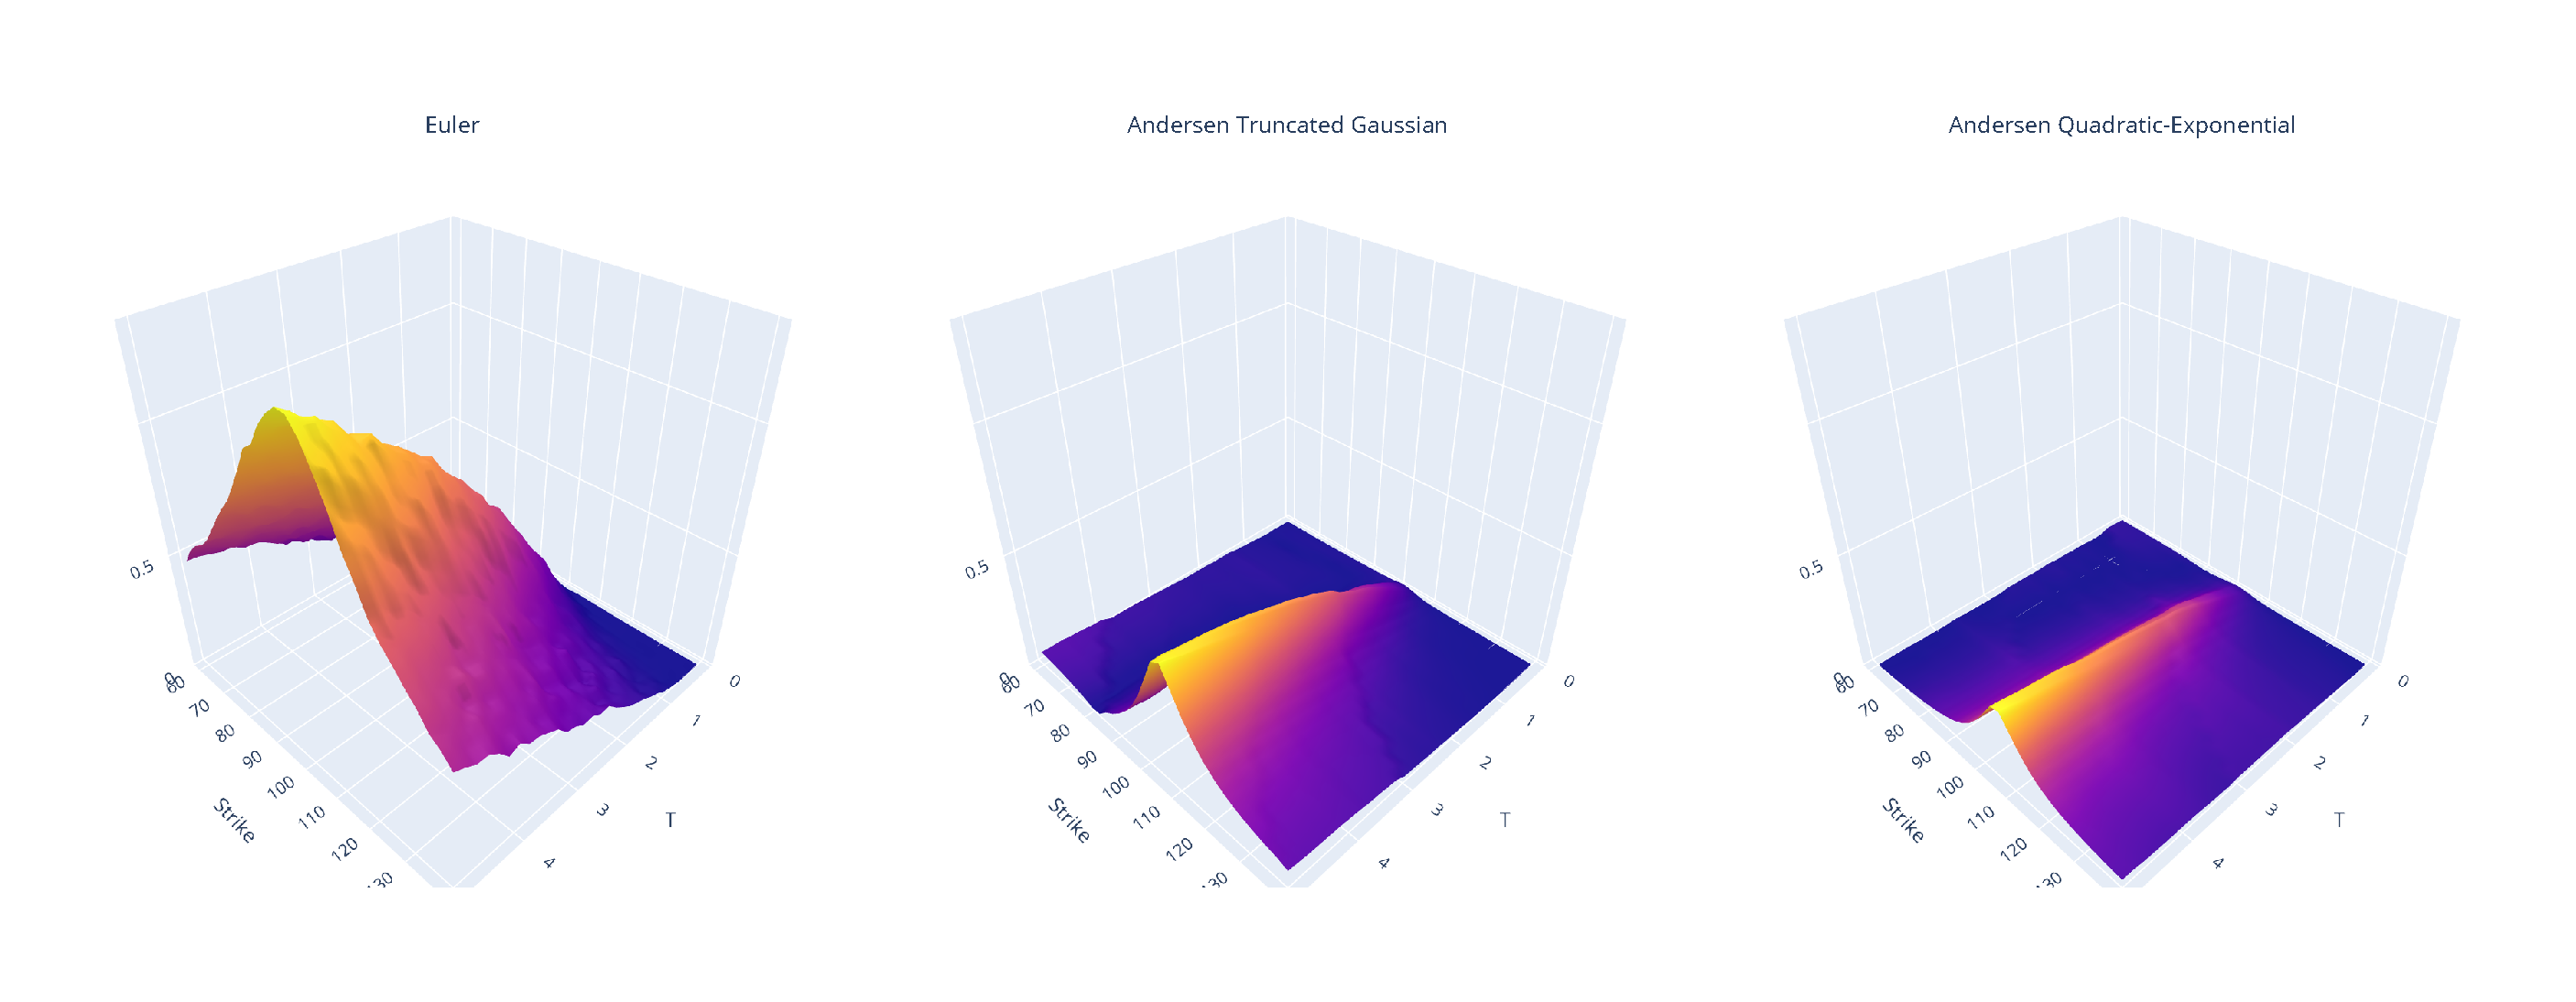
\includegraphics[width=\textwidth]{part4/pictures/err_surface_strike_T_N_T=50_param4.pdf}
        \caption{\texttt{N\_T = 50}, \texttt{absolute\_error = 1e-2}}
    \end{figure}
\end{frame}

\begin{frame}{The Surface of Errors}{Params \#5: $\kappa = 1$, $\gamma = 1$, $\rho = -0.3$, $\bar v = 0.04$, $v_0 = 0.09$}
    \begin{figure}
        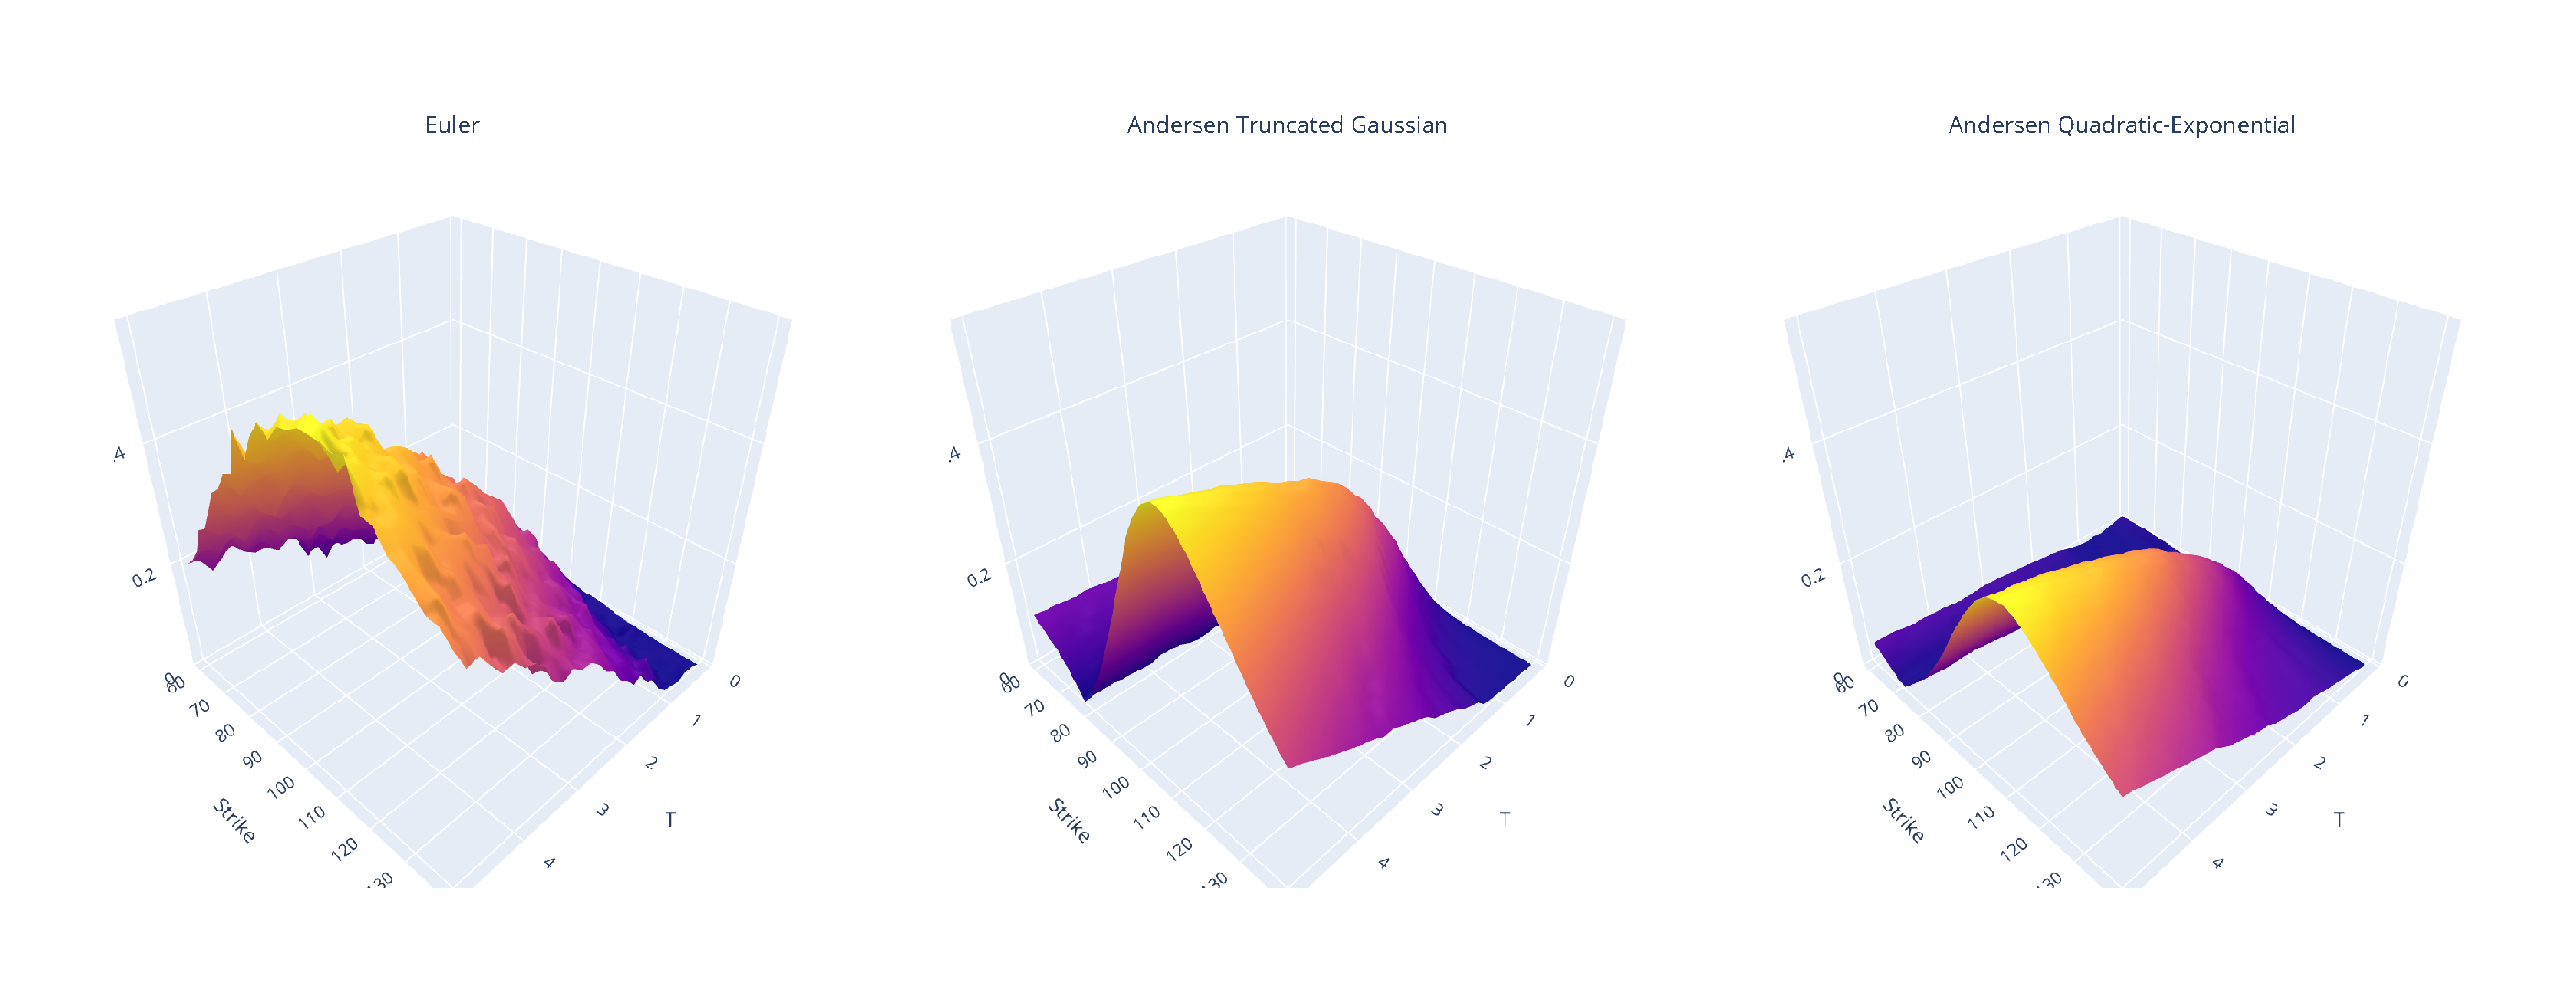
\includegraphics[width=\textwidth]{part4/pictures/err_surface_strike_T_N_T=50_param5.pdf}
        \caption{\texttt{N\_T = 50}, \texttt{absolute\_error = 1e-2}}
    \end{figure}
\end{frame}

\begin{frame}{The Surface of Errors}{Params \#1: $\kappa = 1.3125$, $\gamma = 0.5125$, $\rho = -0.3937$, $\bar v = 0.0641$, $v_0 = 0.3$}
    \begin{figure}
        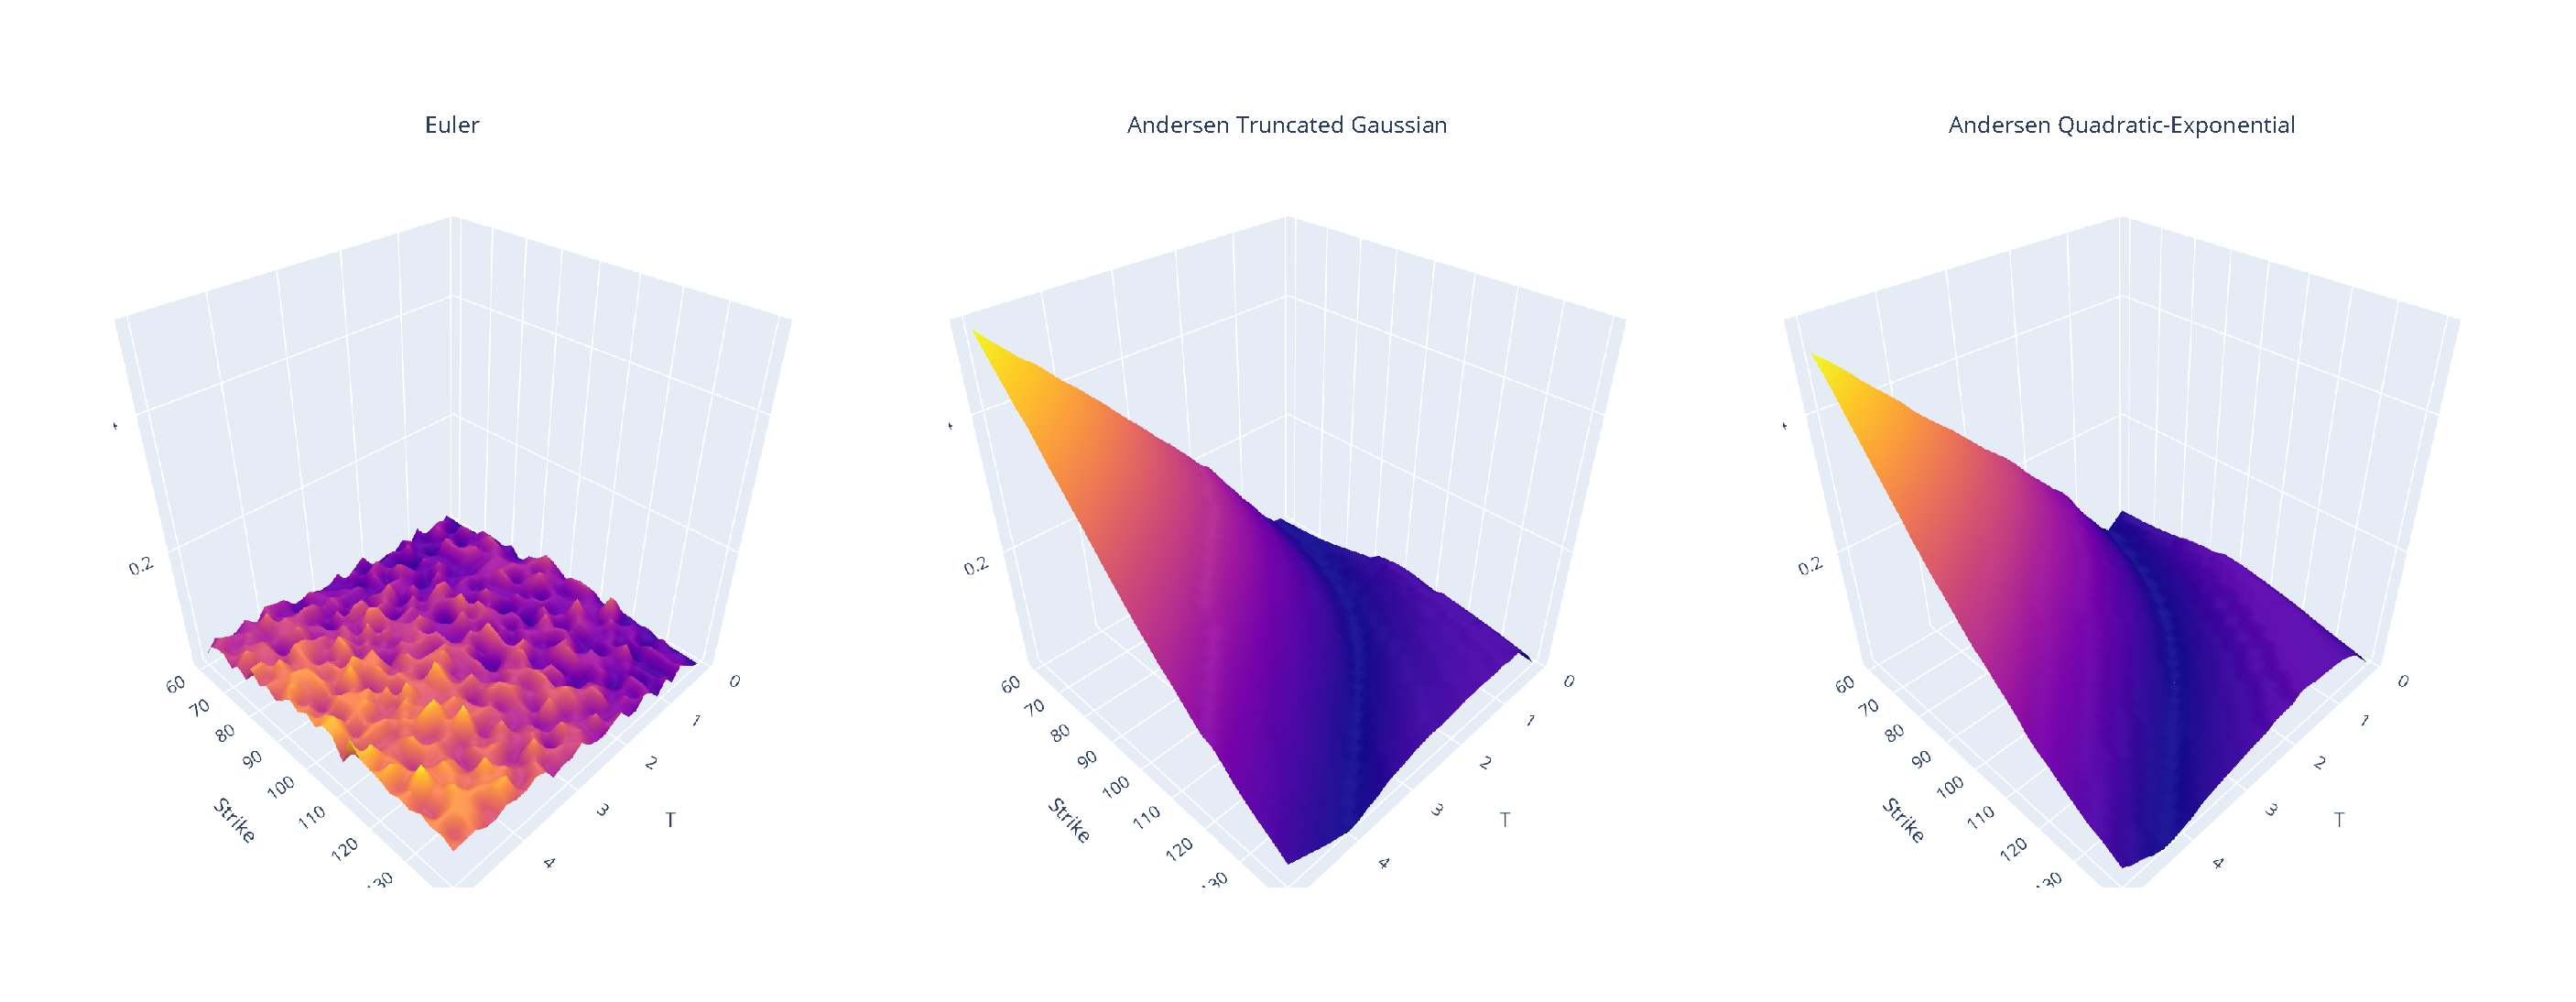
\includegraphics[width=\textwidth]{part4/pictures/err_surface_strike_T_N_T=100_param1.pdf}
        \caption{\texttt{N\_T = 100}, \texttt{absolute\_error = 1e-2}}
    \end{figure}
\end{frame}

\begin{frame}{The Surface of Errors}{Params \#2: $\kappa = 1$, $\gamma = 0.4$, $\rho = -0.1$, $\bar v = 0.2$, $v_0 = 0.2$}
    \begin{figure}
        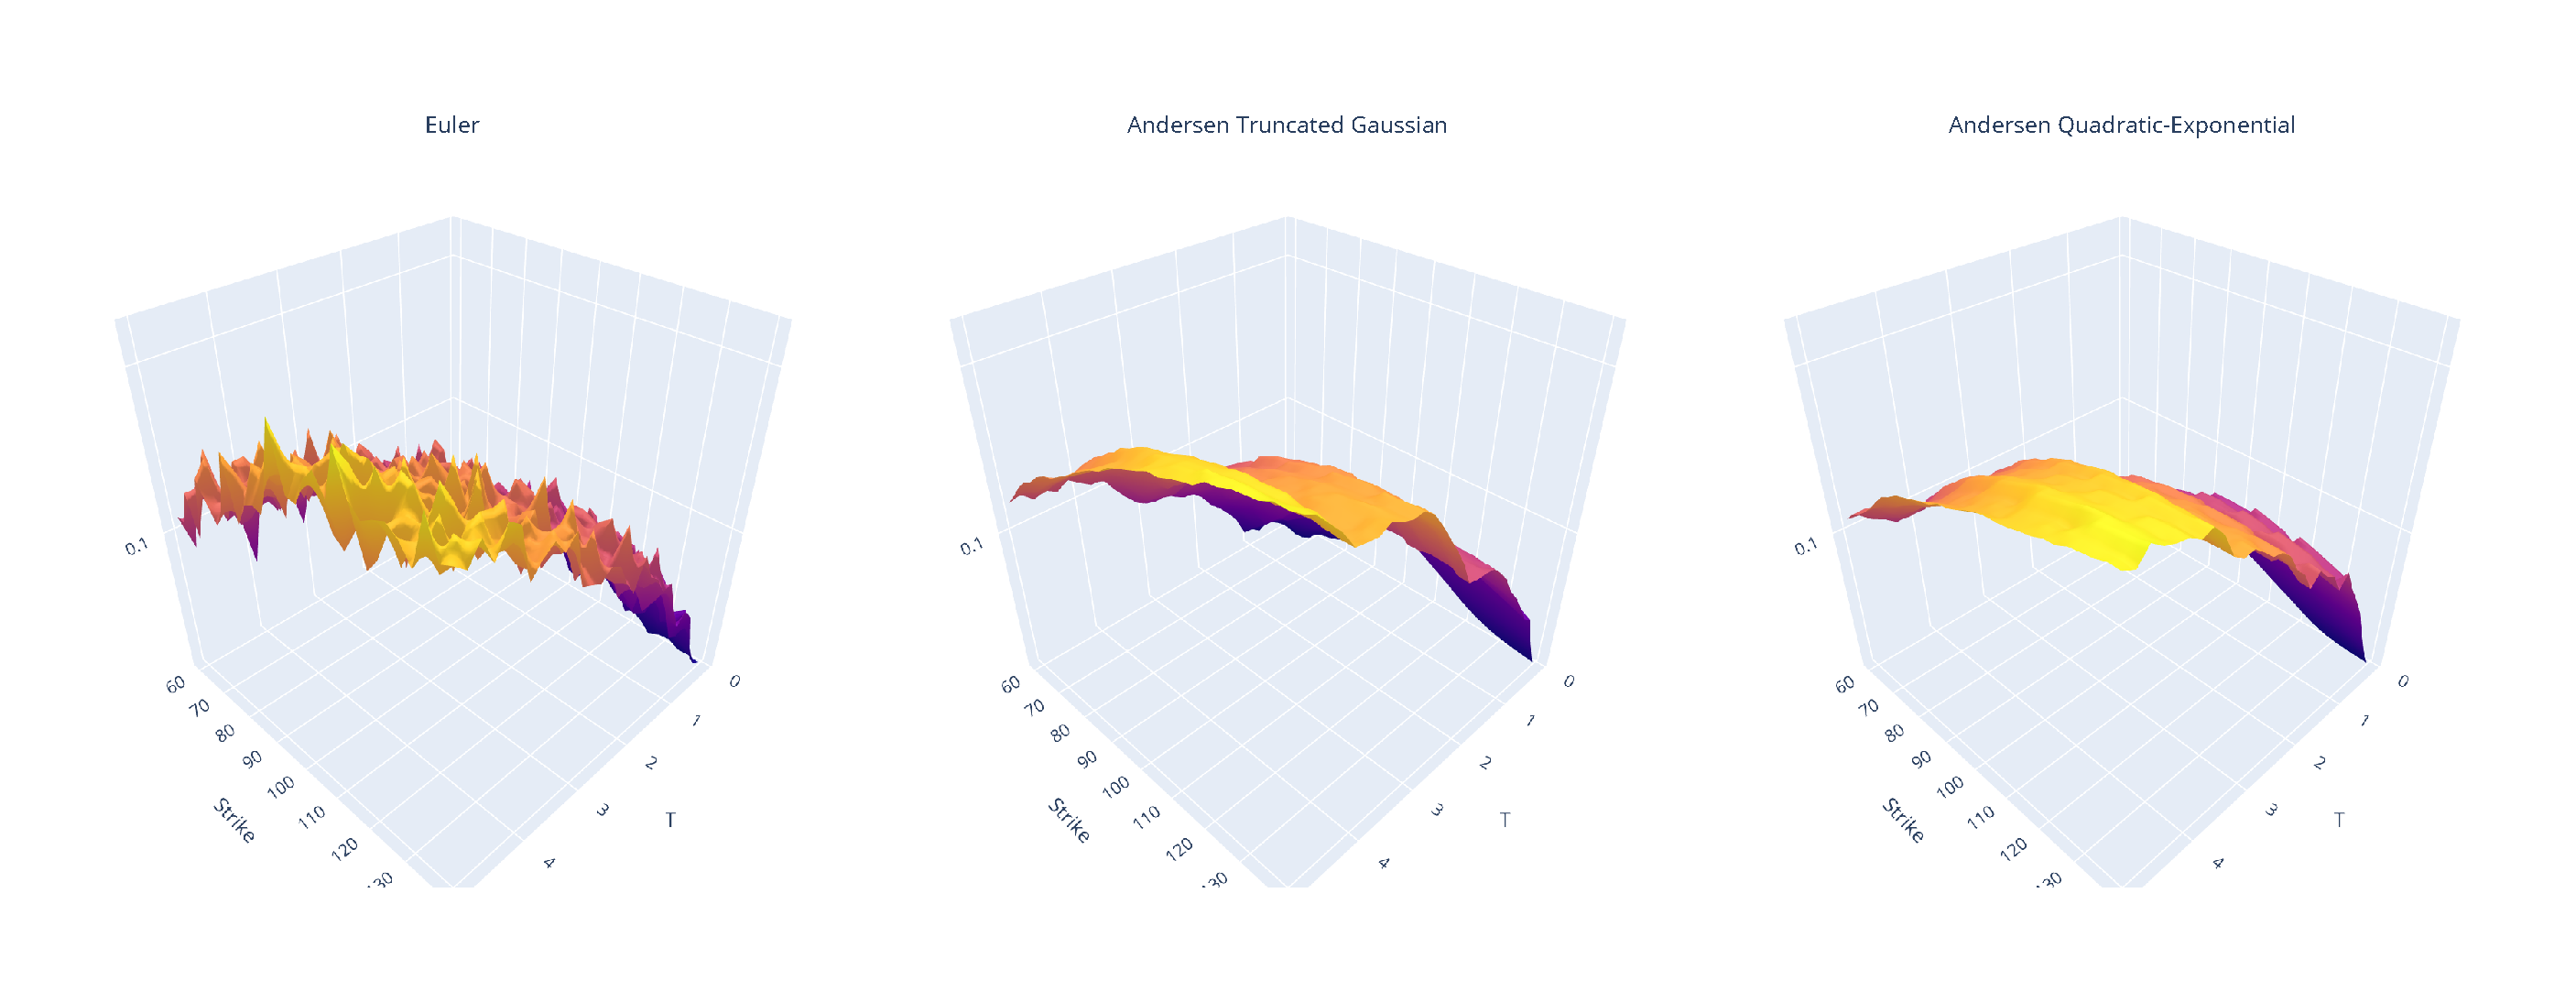
\includegraphics[width=\textwidth]{part4/pictures/err_surface_strike_T_N_T=100_param2.pdf}
        \caption{\texttt{N\_T = 100}, \texttt{absolute\_error = 1e-2}}
    \end{figure}
\end{frame}

\begin{frame}{The Surface of Errors}{Params \#3: $\kappa = 0.5$, $\gamma = 1$, $\rho = -0.9$, $\bar v = 0.04$, $v_0 = 0.04$}
    \begin{figure}
        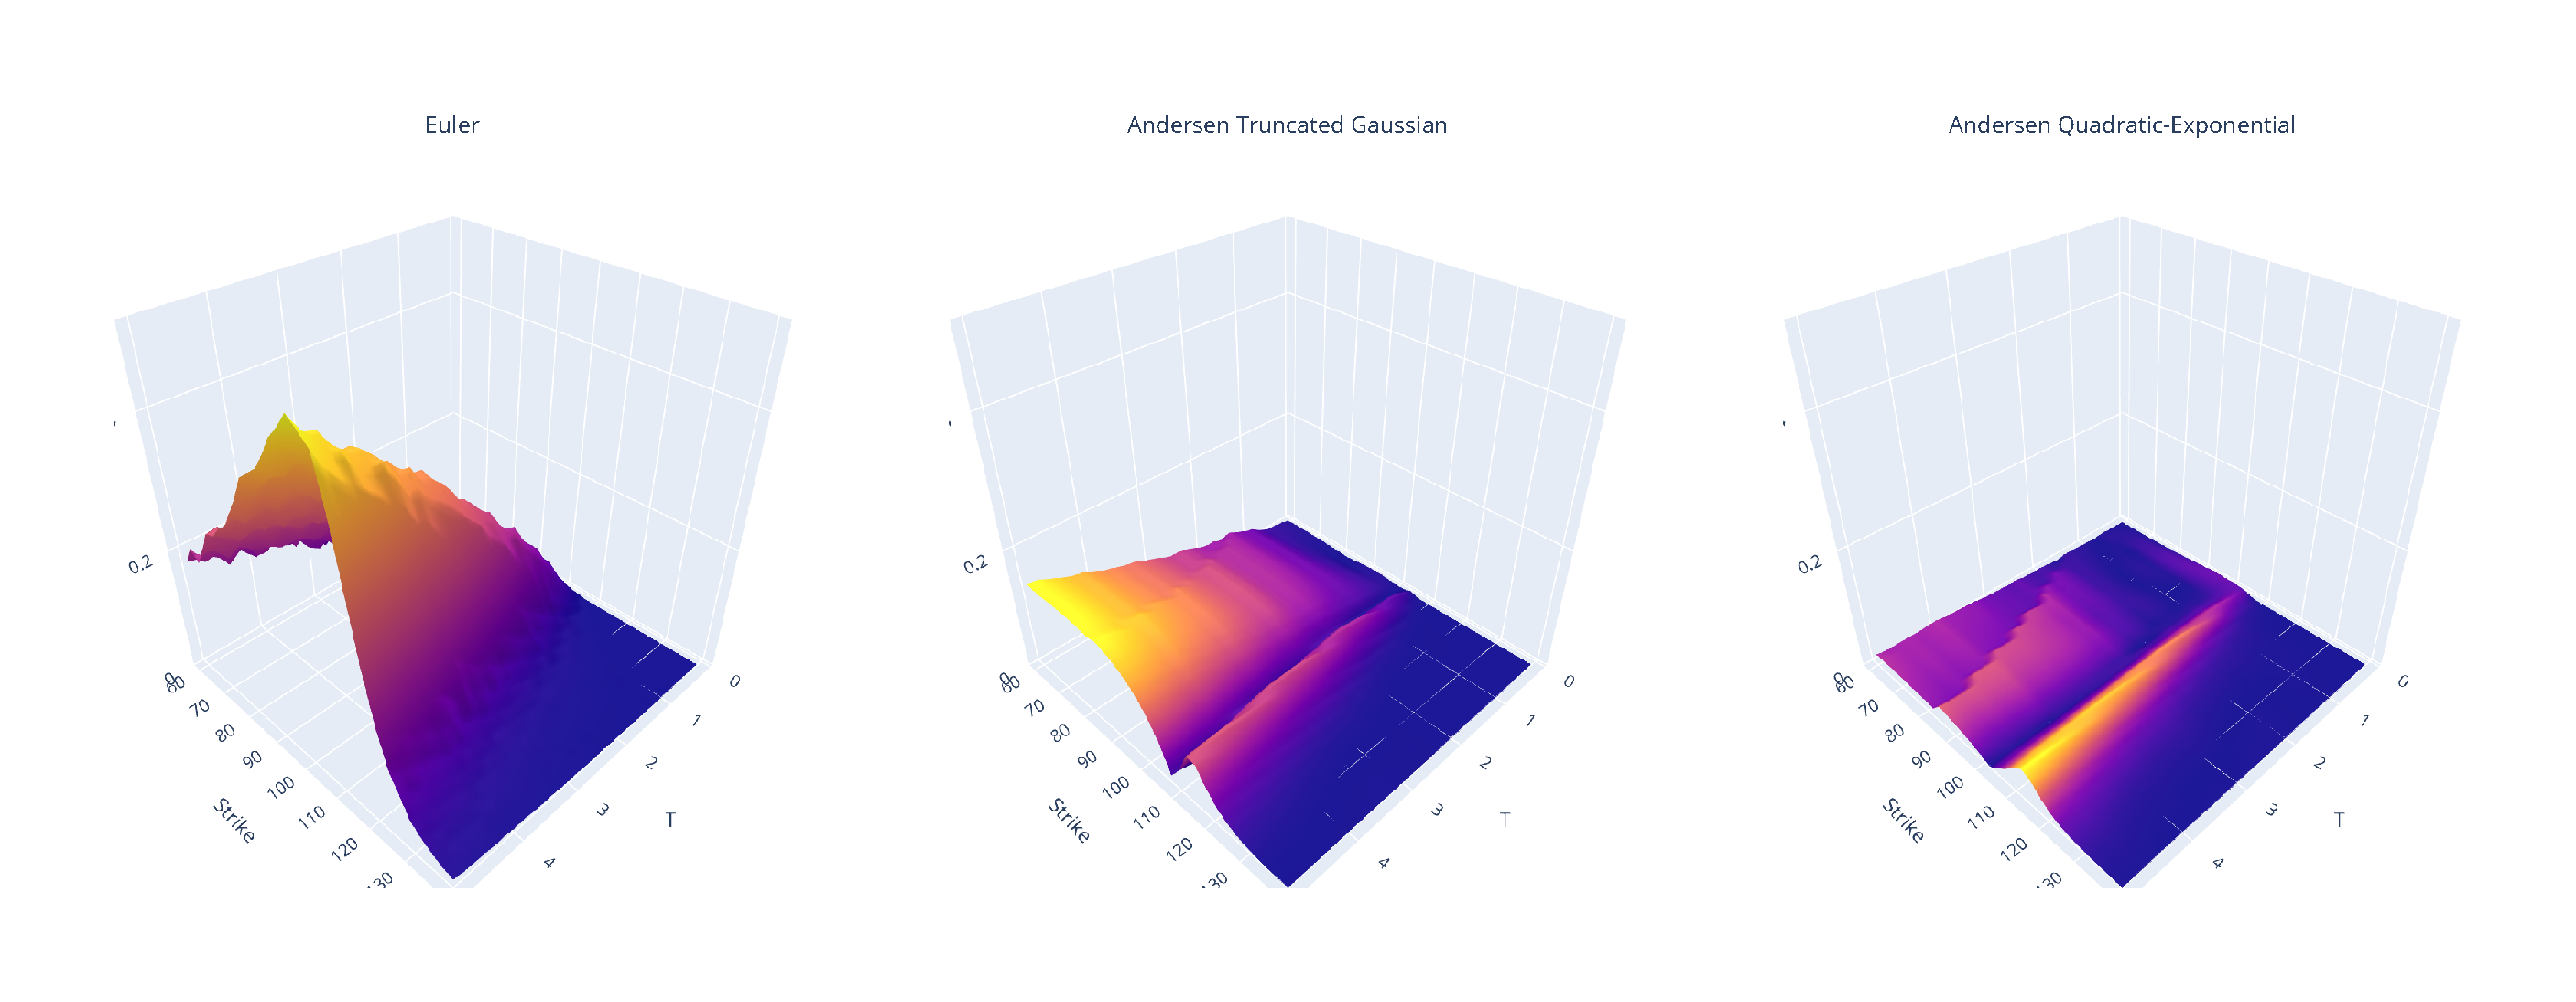
\includegraphics[width=\textwidth]{part4/pictures/err_surface_strike_T_N_T=100_param3.pdf}
        \caption{\texttt{N\_T = 100}, \texttt{absolute\_error = 1e-2}}
    \end{figure}
\end{frame}

\begin{frame}{The Surface of Errors}{Params \#4: $\kappa = 0.3$, $\gamma = 0.9$, $\rho = -0.5$, $\bar v = 0.04$, $v_0 = 0.04$}
    \begin{figure}
        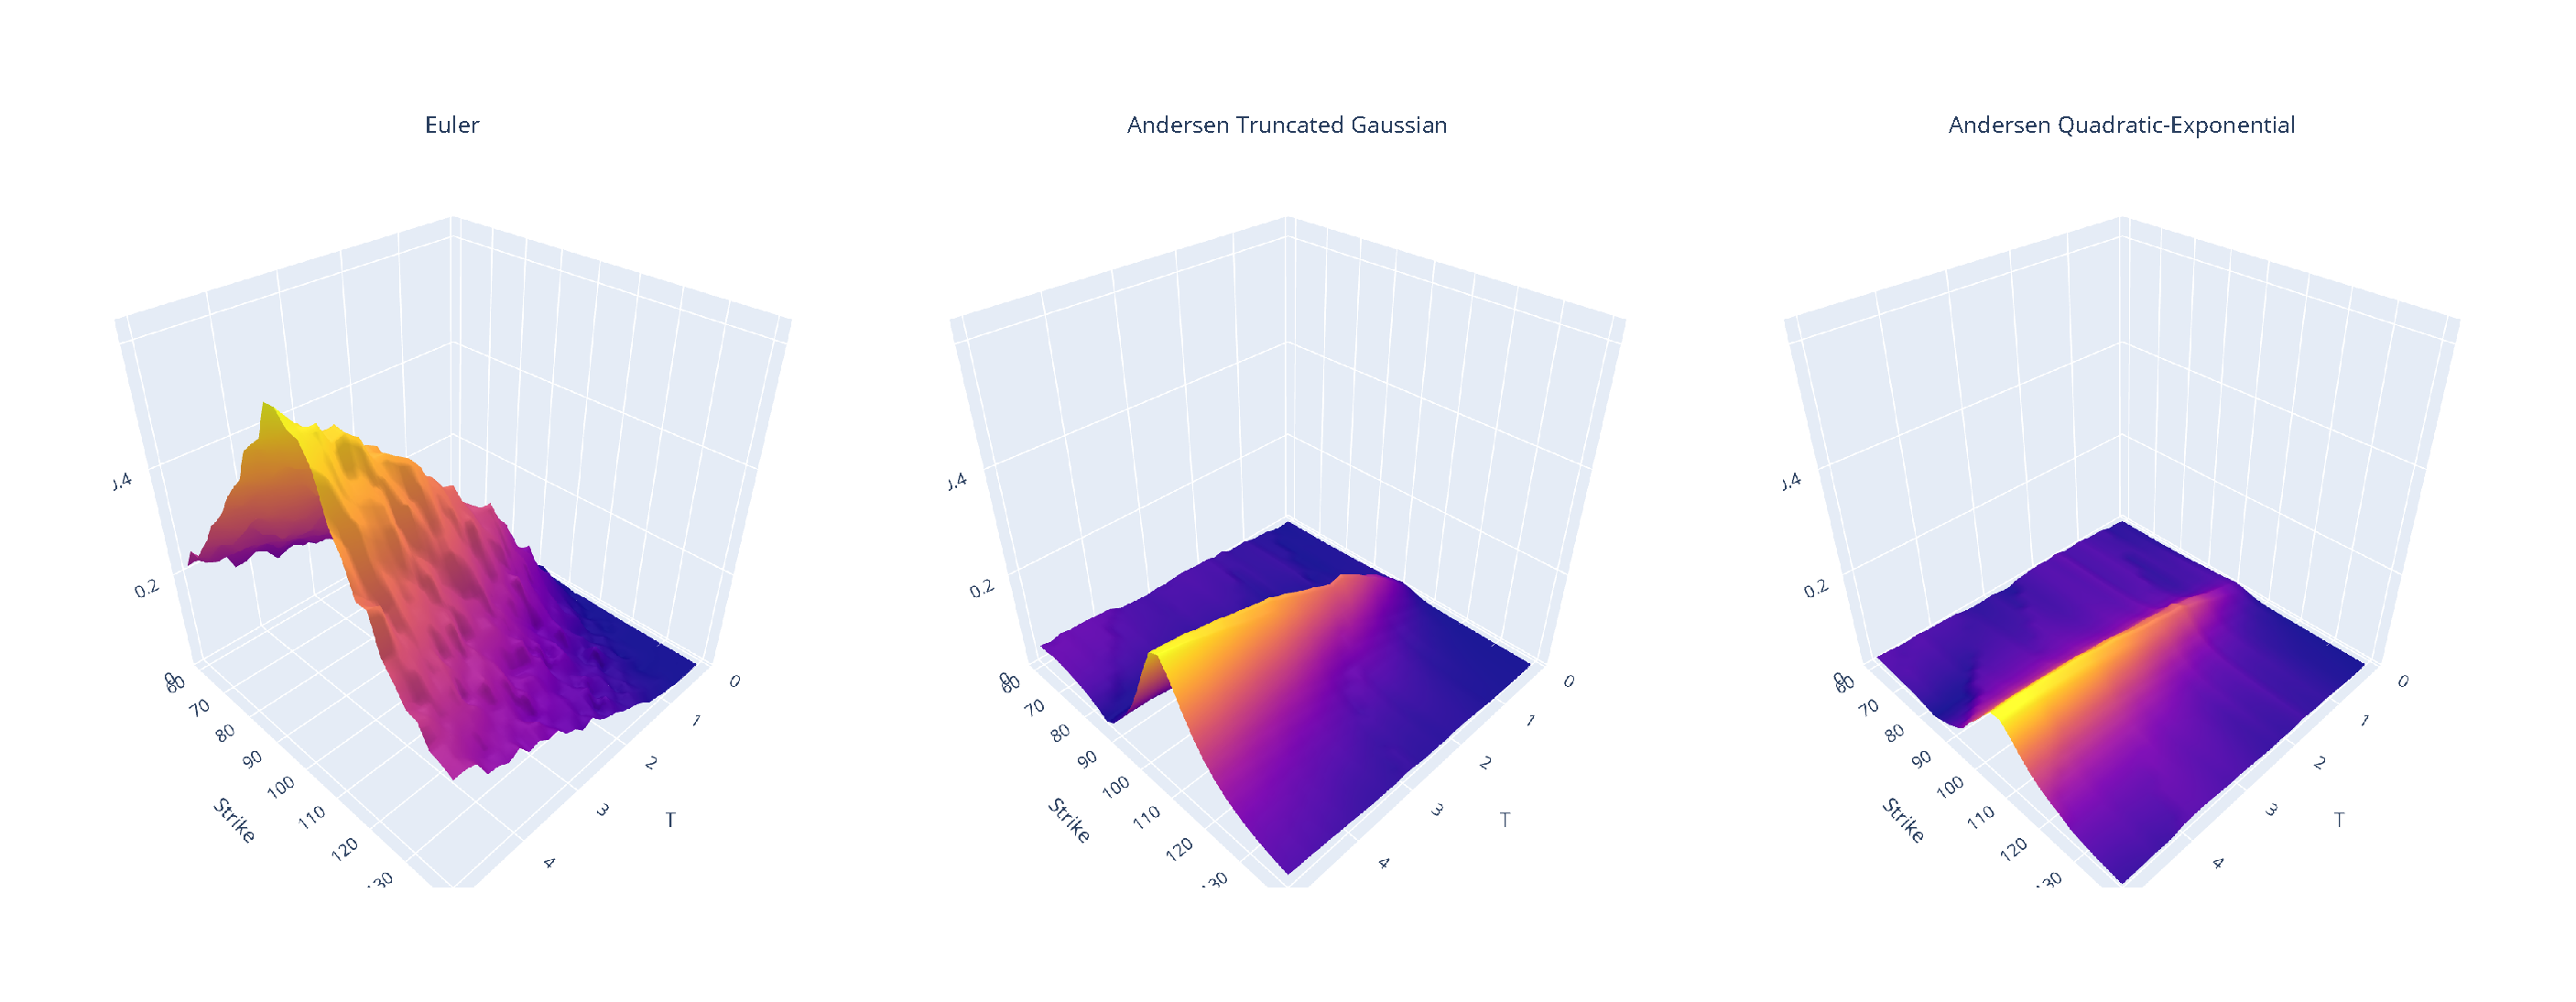
\includegraphics[width=\textwidth]{part4/pictures/err_surface_strike_T_N_T=100_param4.pdf}
        \caption{\texttt{N\_T = 100}, \texttt{absolute\_error = 1e-2}}
    \end{figure}
\end{frame}

\begin{frame}{The Surface of Errors}{Params \#5: $\kappa = 1$, $\gamma = 1$, $\rho = -0.3$, $\bar v = 0.04$, $v_0 = 0.09$}
    \begin{figure}
        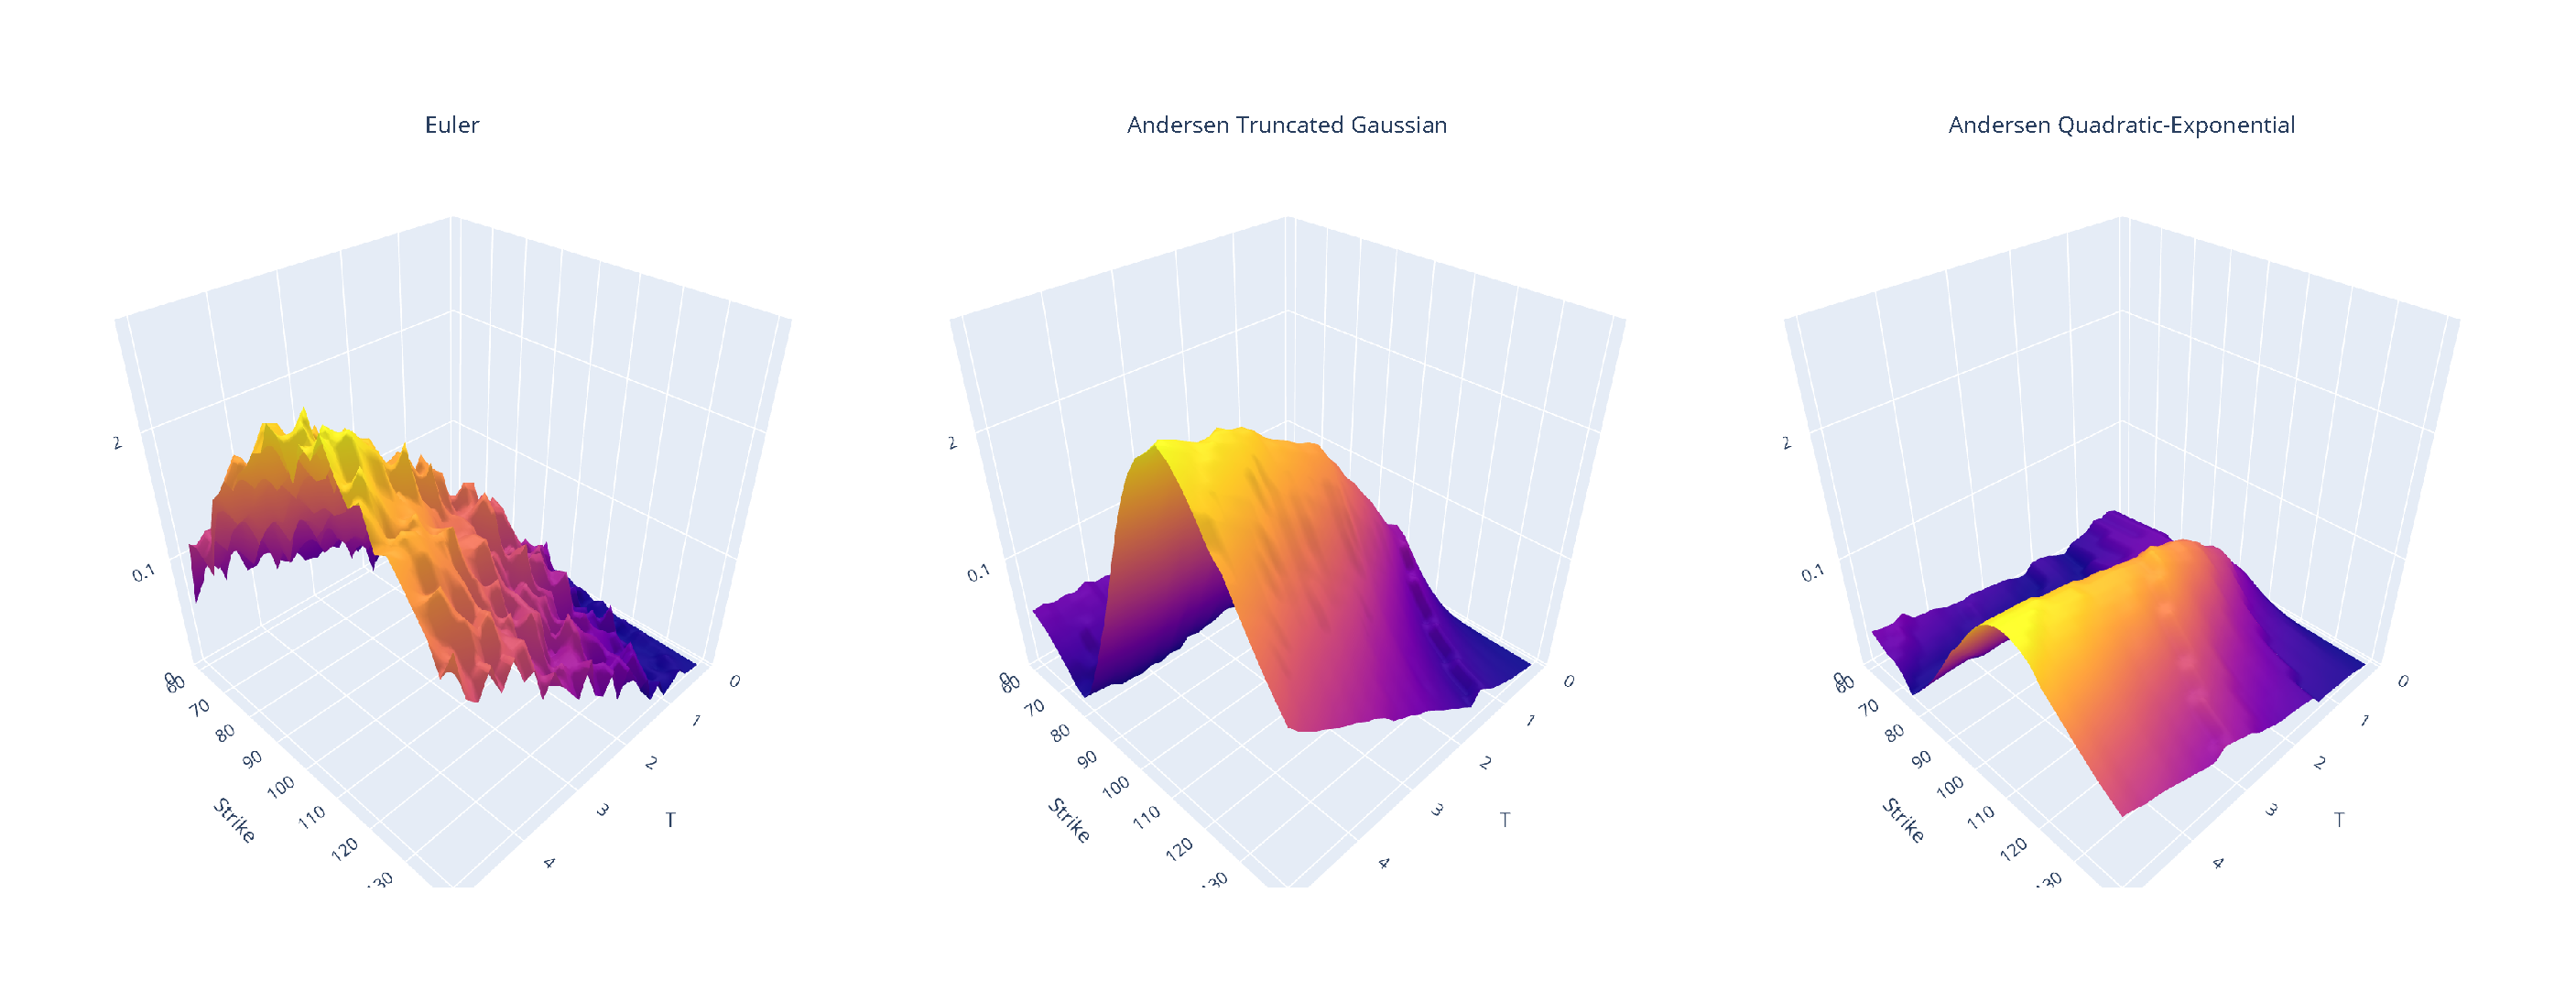
\includegraphics[width=\textwidth]{part4/pictures/err_surface_strike_T_N_T=100_param5.pdf}
        \caption{\texttt{N\_T = 100}, \texttt{absolute\_error = 1e-2}}
    \end{figure}
\end{frame}

\begin{frame}{Speed Boost compared to the Euler Scheme}{Params \#3: $\kappa = 0.5$, $\gamma = 1$, $\rho = -0.9$, $\bar v = 0.04$, $v_0 = 0.04$}
    \begin{figure}
        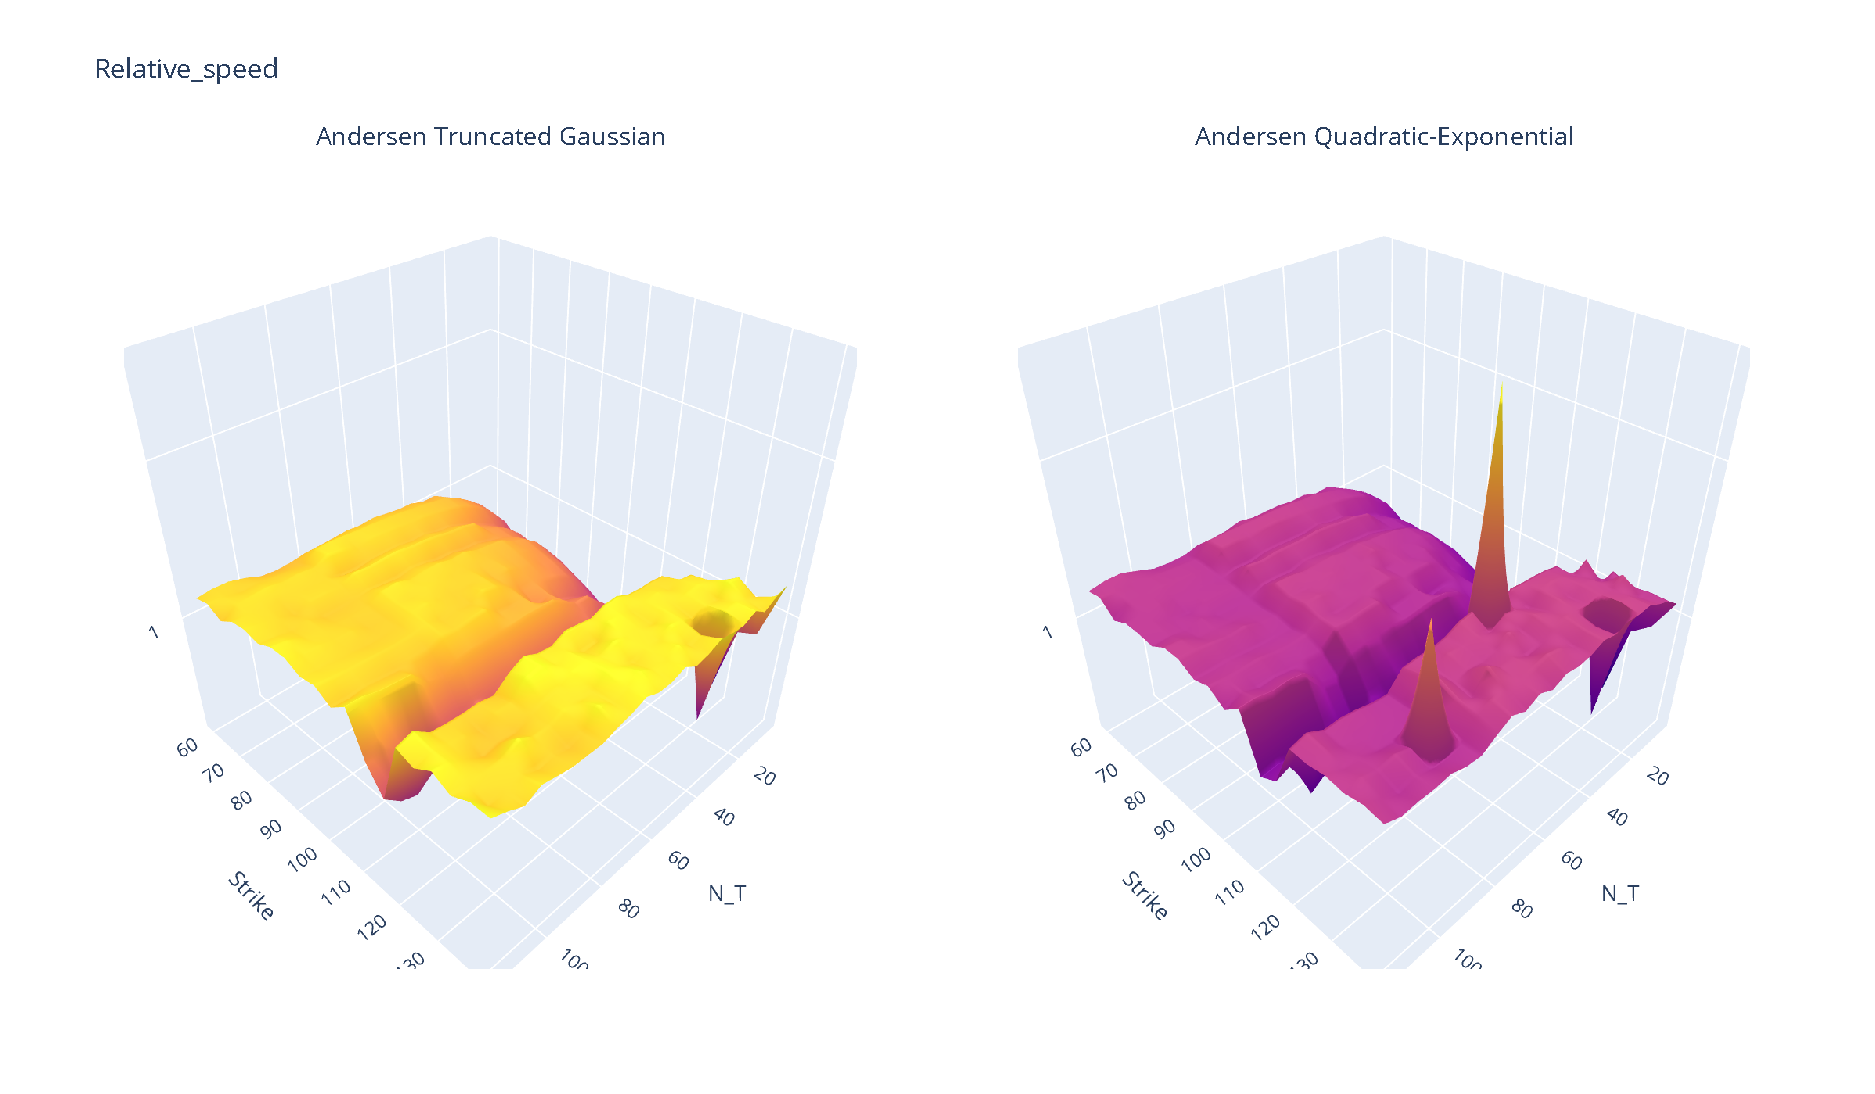
\includegraphics[width=0.9\textwidth]{part4/pictures/relative_speed_strike_N_T.pdf}
    \end{figure}
\end{frame}




    \section{Variance Reduction Methods Efficiency}
        \subsection{Control Variates}
    \begin{frame}{Control Variates}{Params \#3: $\kappa = 0.5$, $\gamma = 1$, $\rho = -0.9$, $\bar v = 0.04$, $v_0 = 0.04$, \texttt{absolute\_error = 5e-2}}
        \begin{figure}
            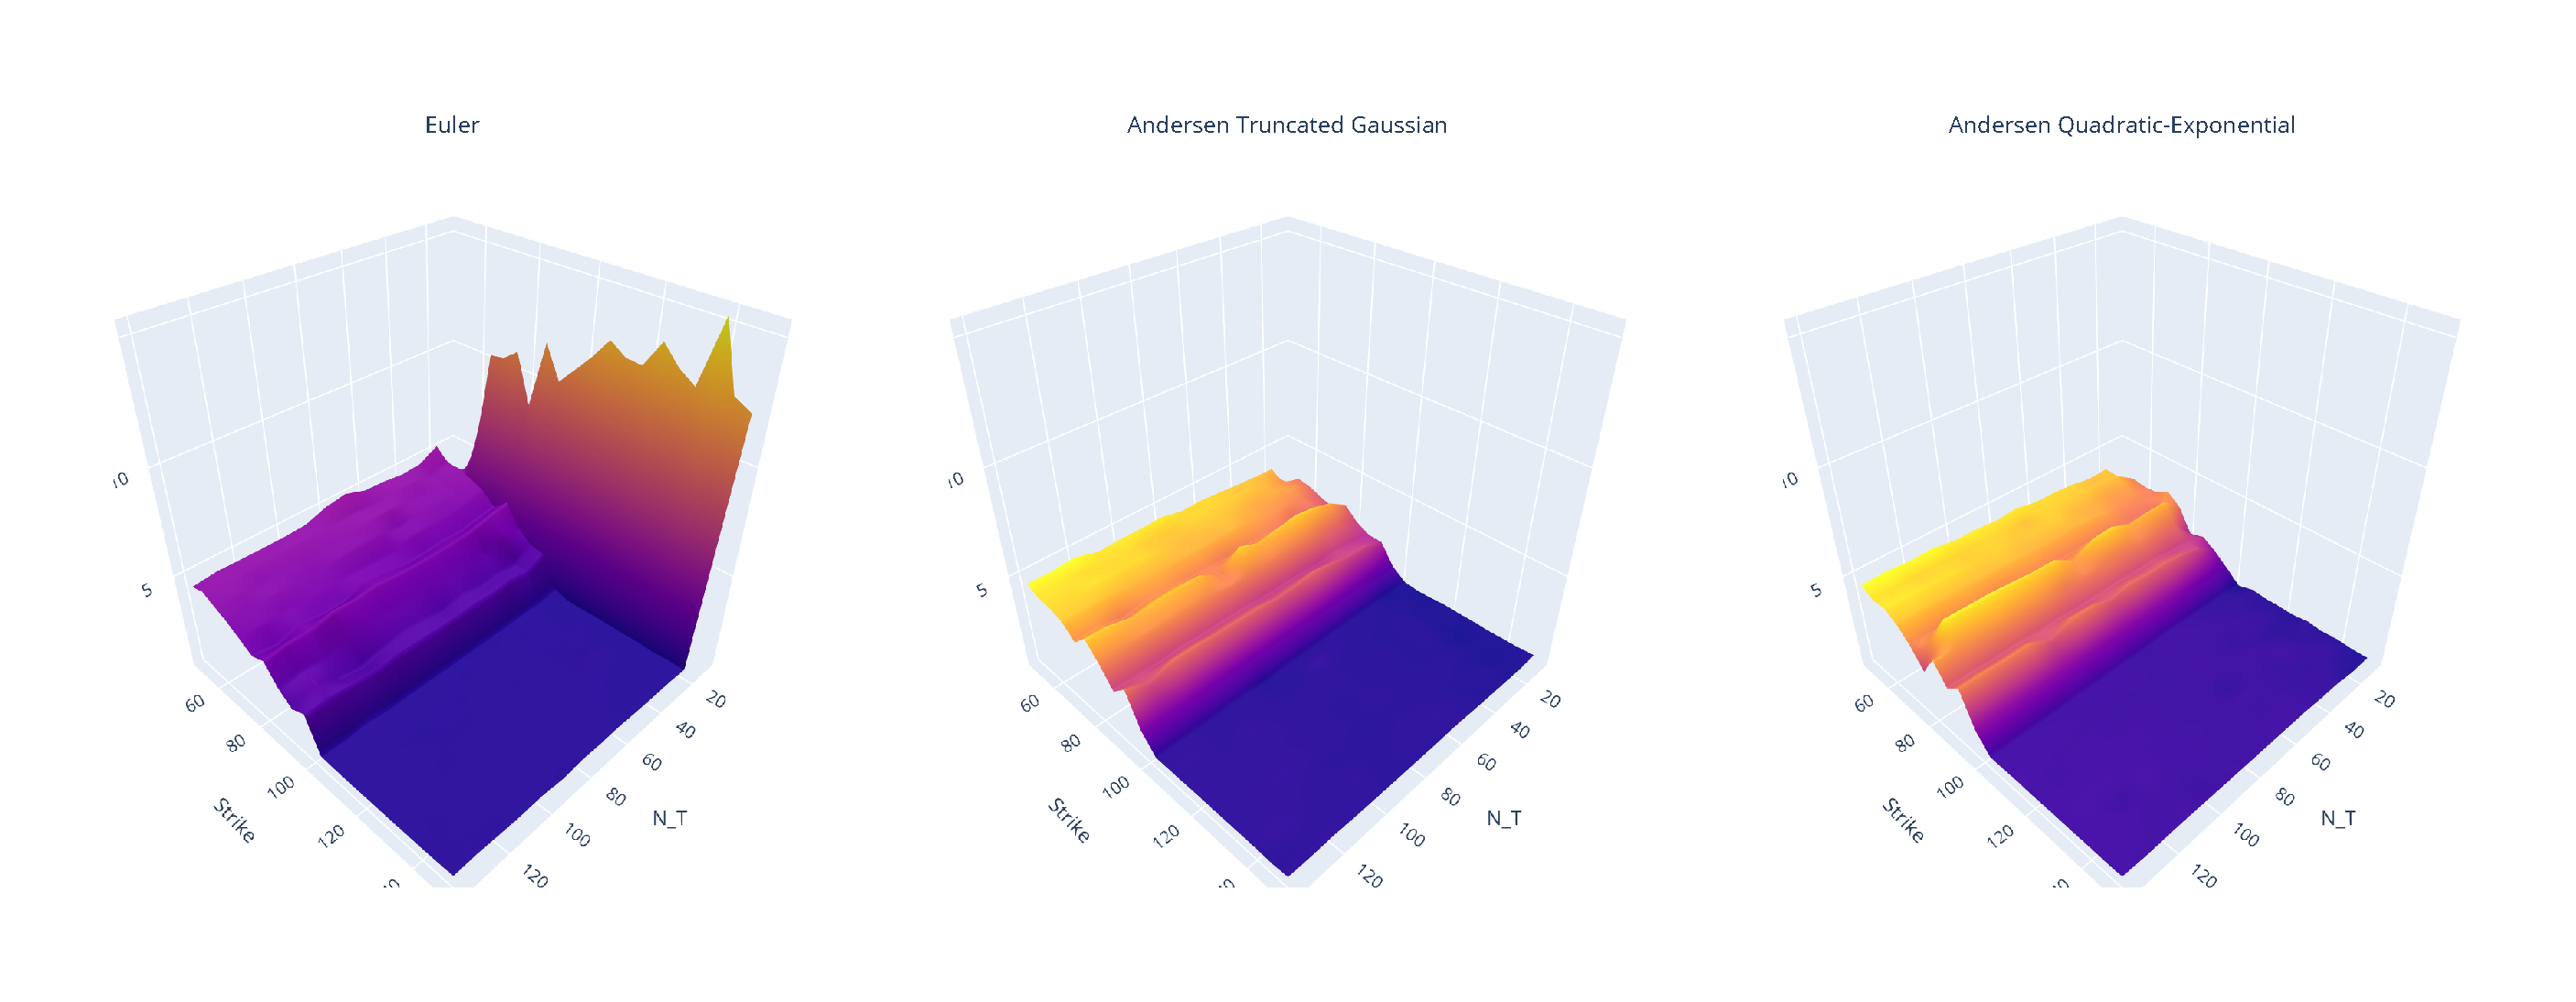
\includegraphics[width=\textwidth]{part5/pictures/surf_3.pdf}
        \end{figure}
    \end{frame}

    \begin{frame}{Control Variates}{Params \#3: $\kappa = 0.5$, $\gamma = 1$, $\rho = -0.9$, $\bar v = 0.04$, $v_0 = 0.04$, \texttt{absolute\_error = 5e-2}}
        \begin{figure}
            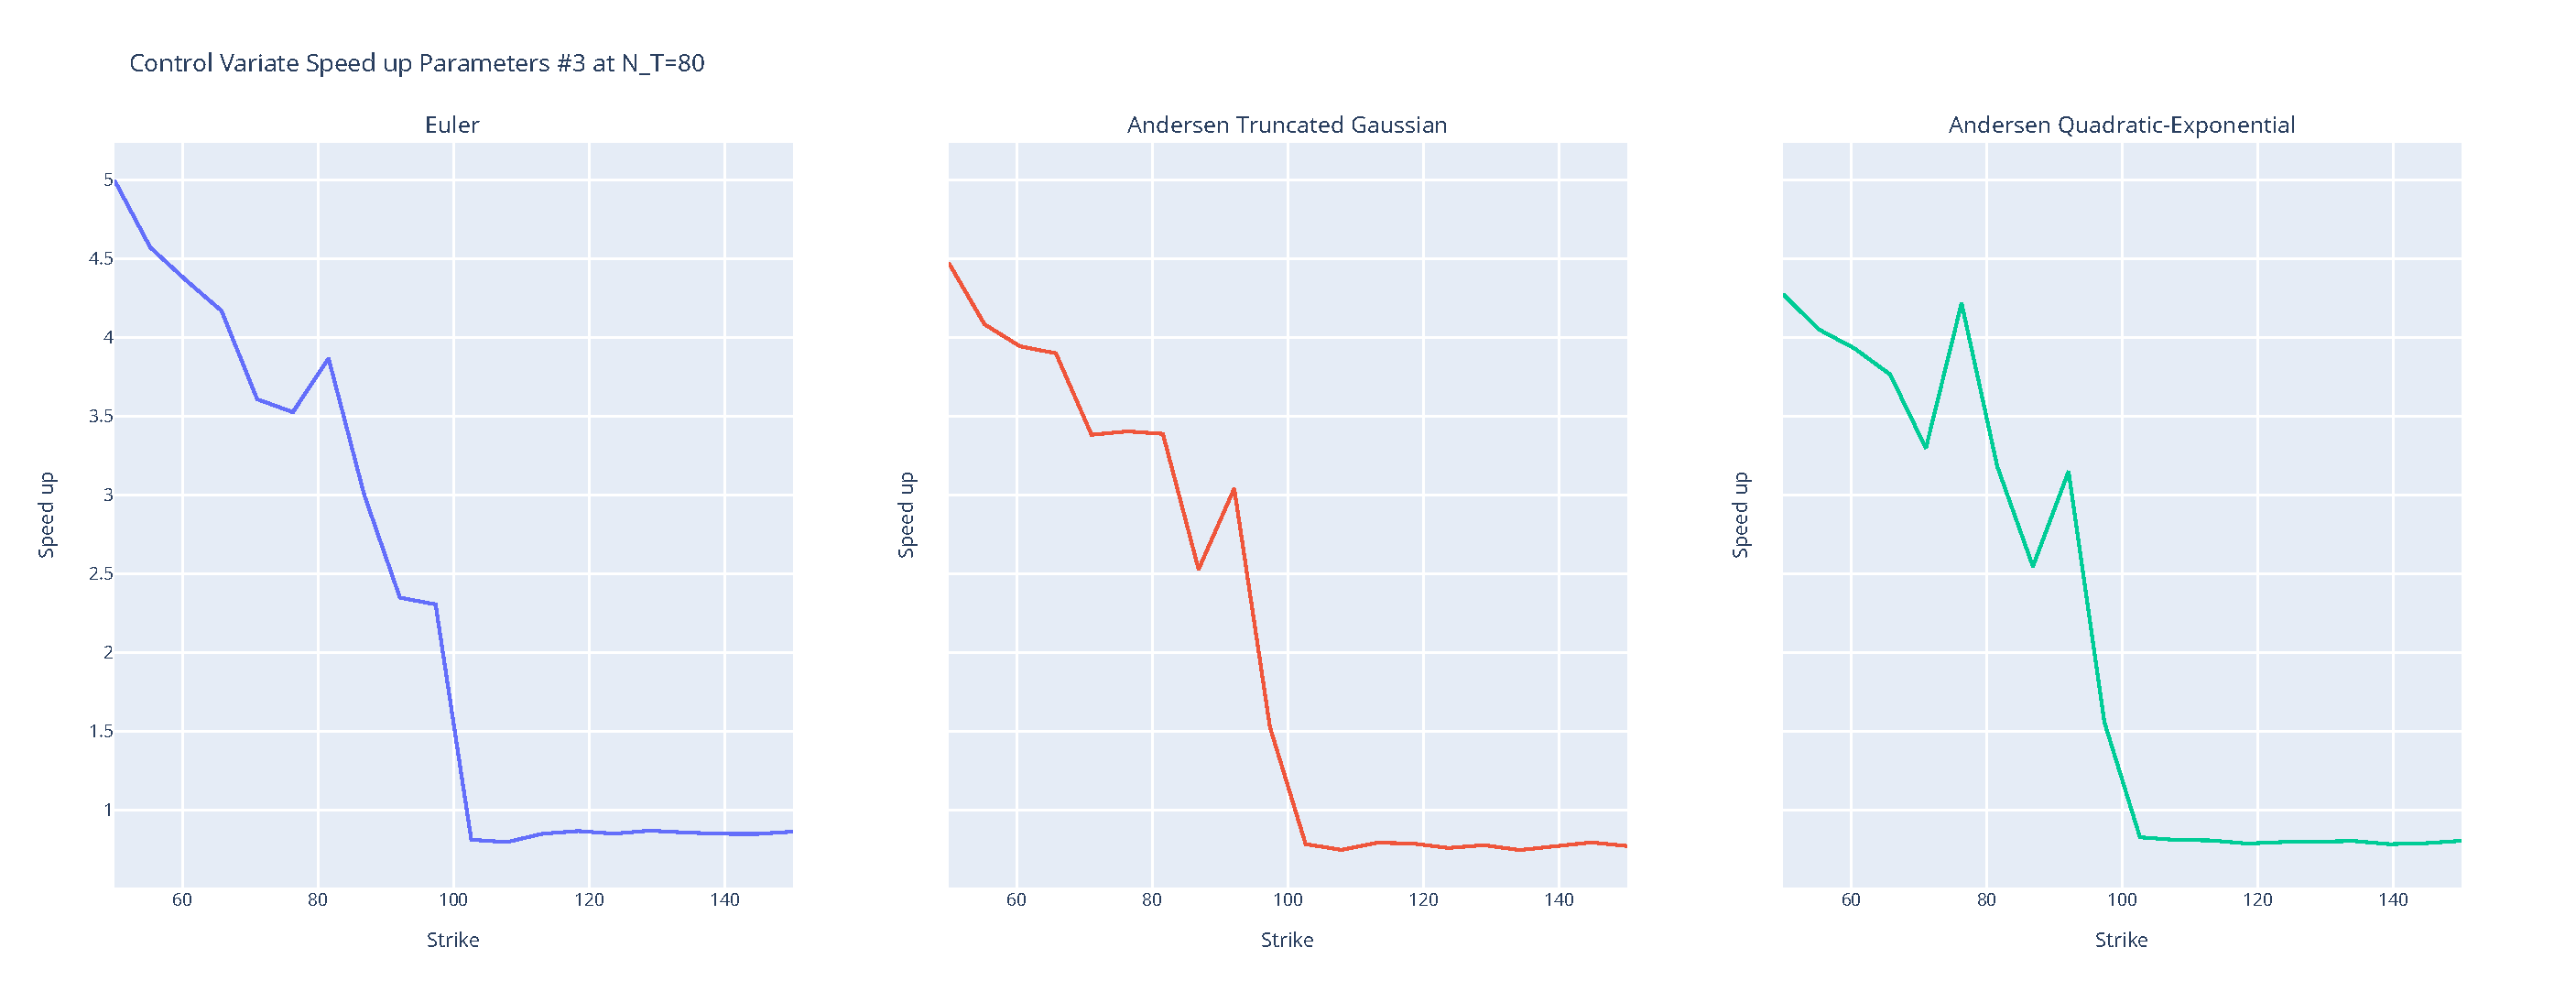
\includegraphics[width=\textwidth]{part5/pictures/pot_3.pdf}
        \end{figure}
    \end{frame}

    \begin{frame}{Control Variates}{Params \#4: $\kappa = 0.3$, $\gamma = 0.9$, $\rho = -0.5$, $\bar v = 0.04$, $v_0 = 0.04$, \texttt{absolute\_error = 5e-2}}
        \begin{figure}
            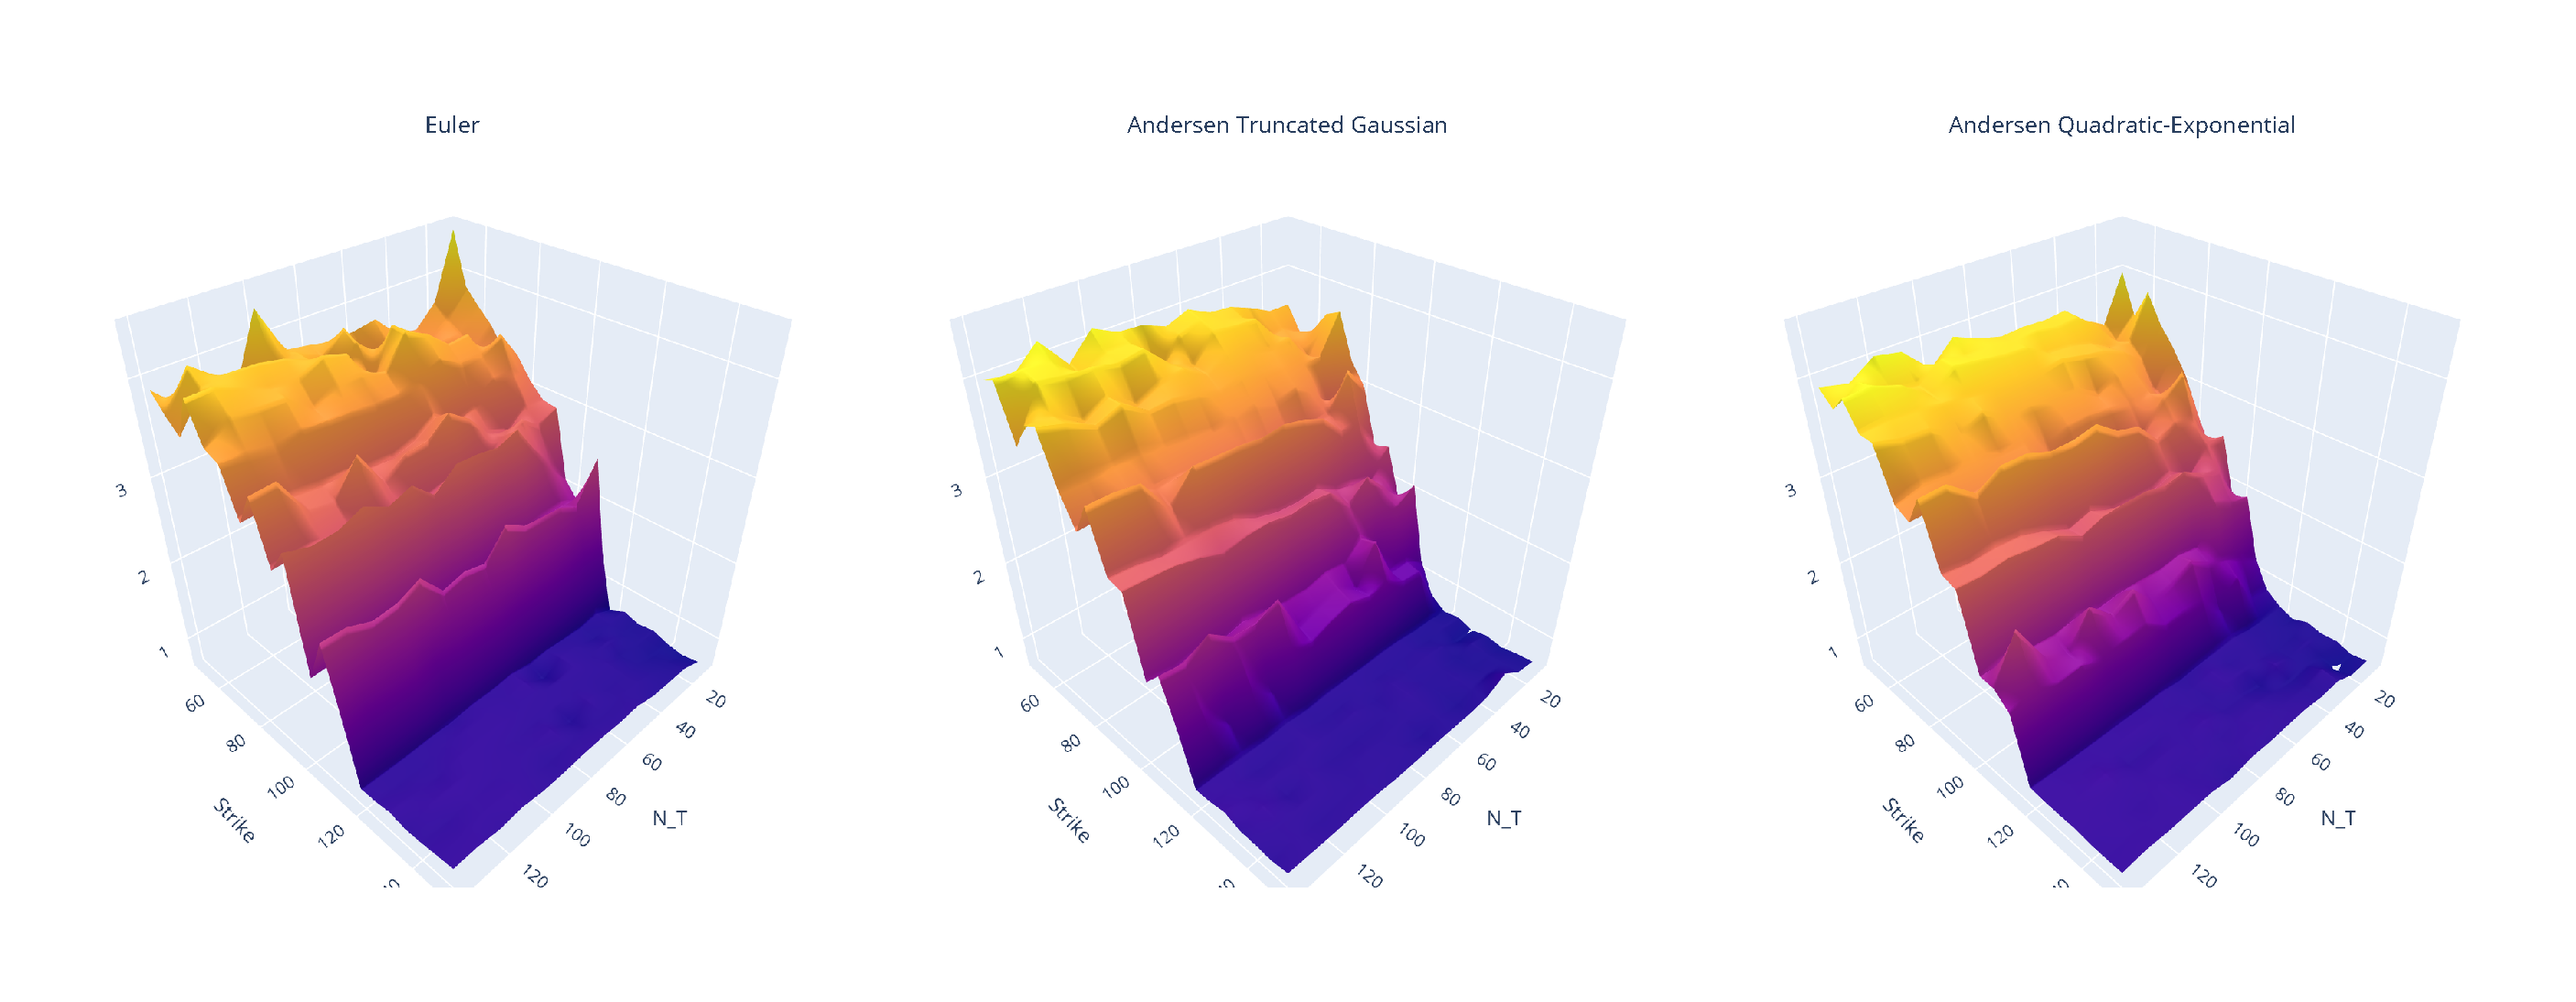
\includegraphics[width=\textwidth]{part5/pictures/surf_4.pdf}
        \end{figure}
    \end{frame}

    \begin{frame}{Control Variates}{Params \#4: $\kappa = 0.3$, $\gamma = 0.9$, $\rho = -0.5$, $\bar v = 0.04$, $v_0 = 0.04$, \texttt{absolute\_error = 5e-2}}
        \begin{figure}
            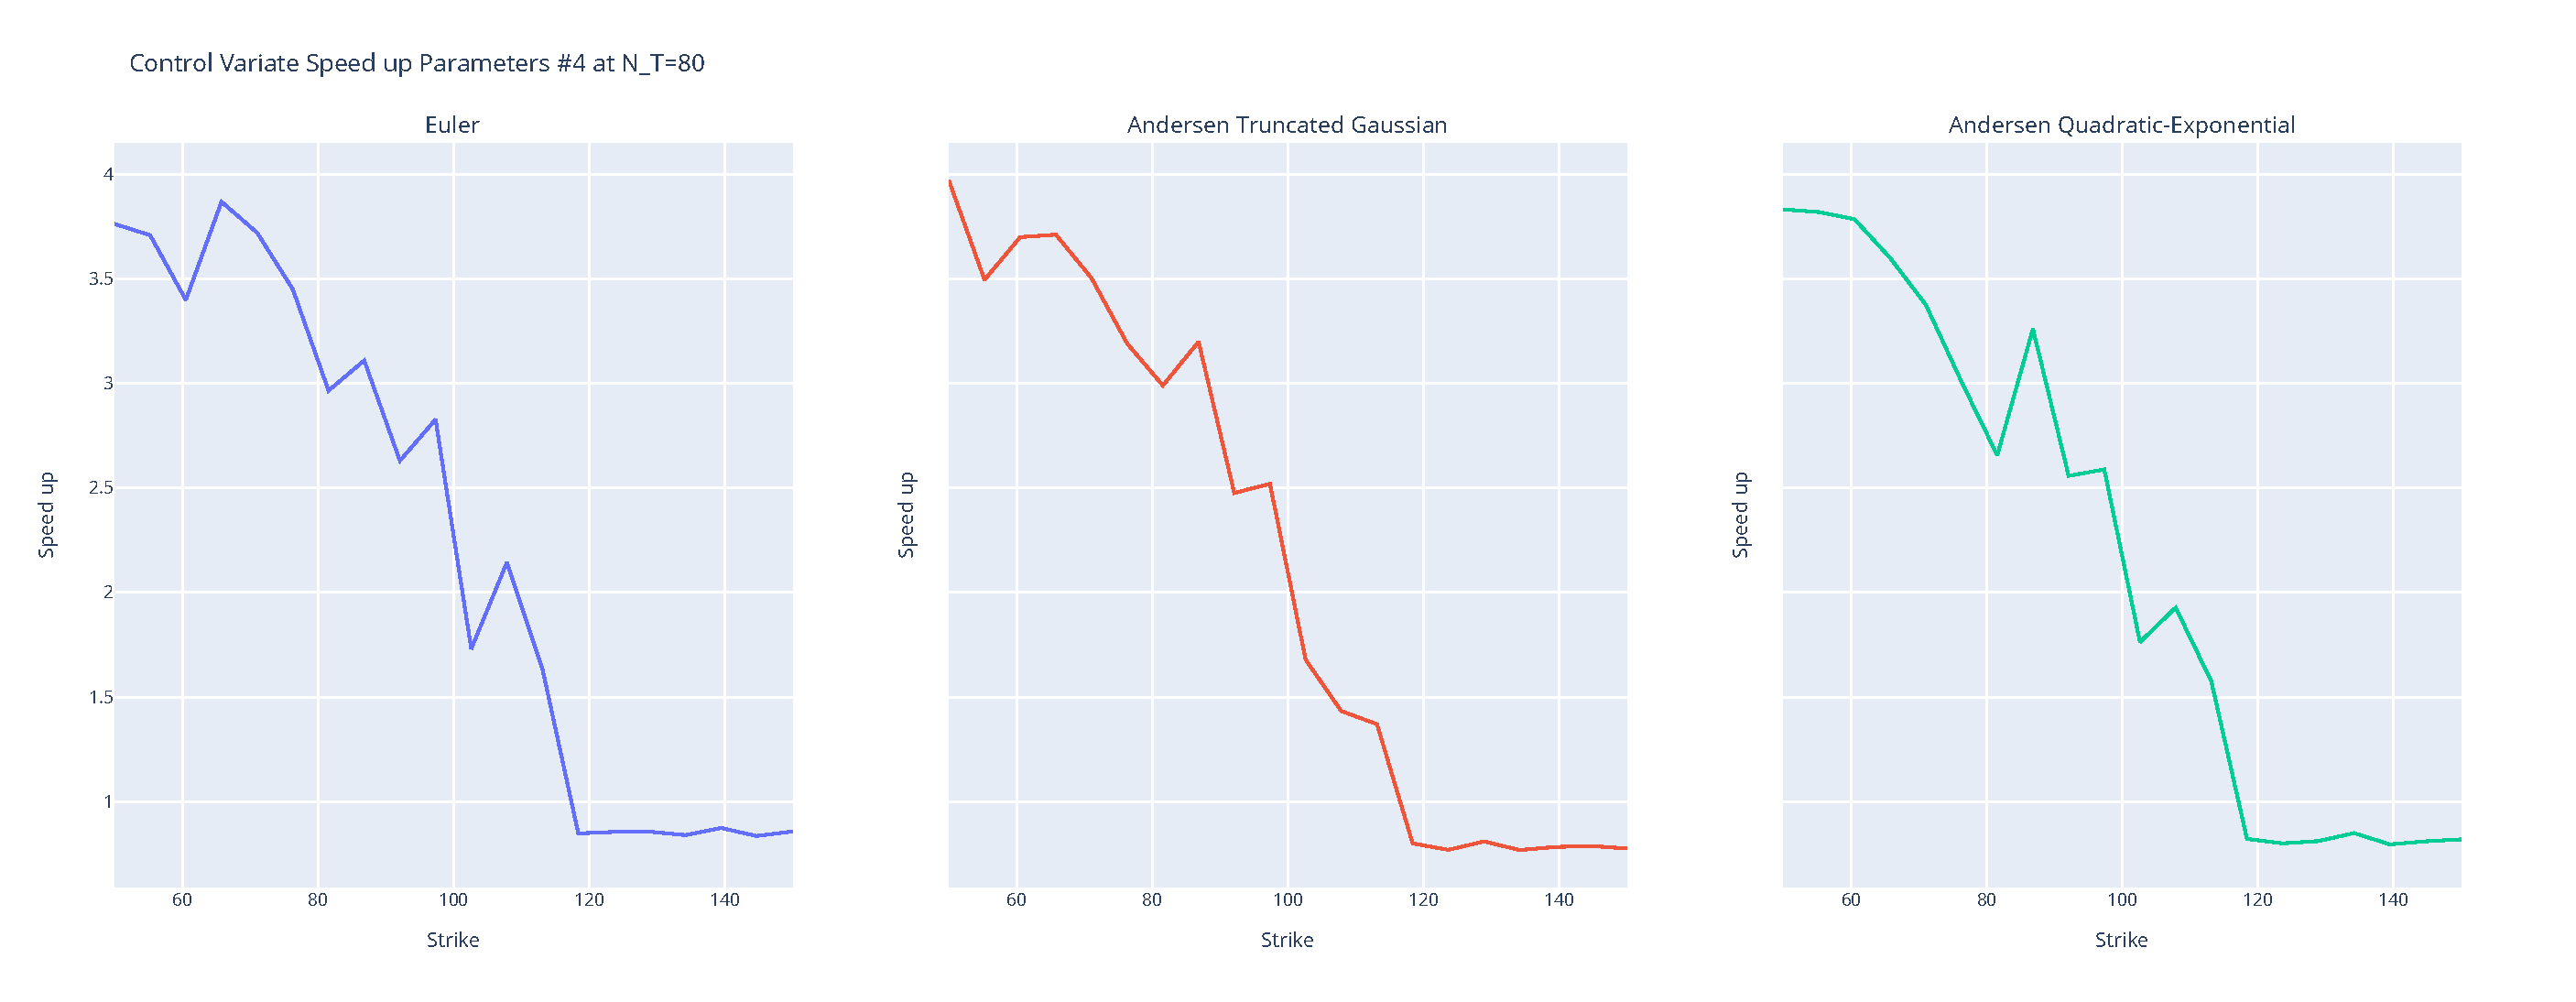
\includegraphics[width=\textwidth]{part5/pictures/pot_4.pdf}
        \end{figure}
    \end{frame}

    \begin{frame}{Control Variates}{Params \#5: $\kappa = 1$, $\gamma = 1$, $\rho = -0.3$, $\bar v = 0.04$, $v_0 = 0.09$, \texttt{absolute\_error = 5e-2}}
        \begin{figure}
            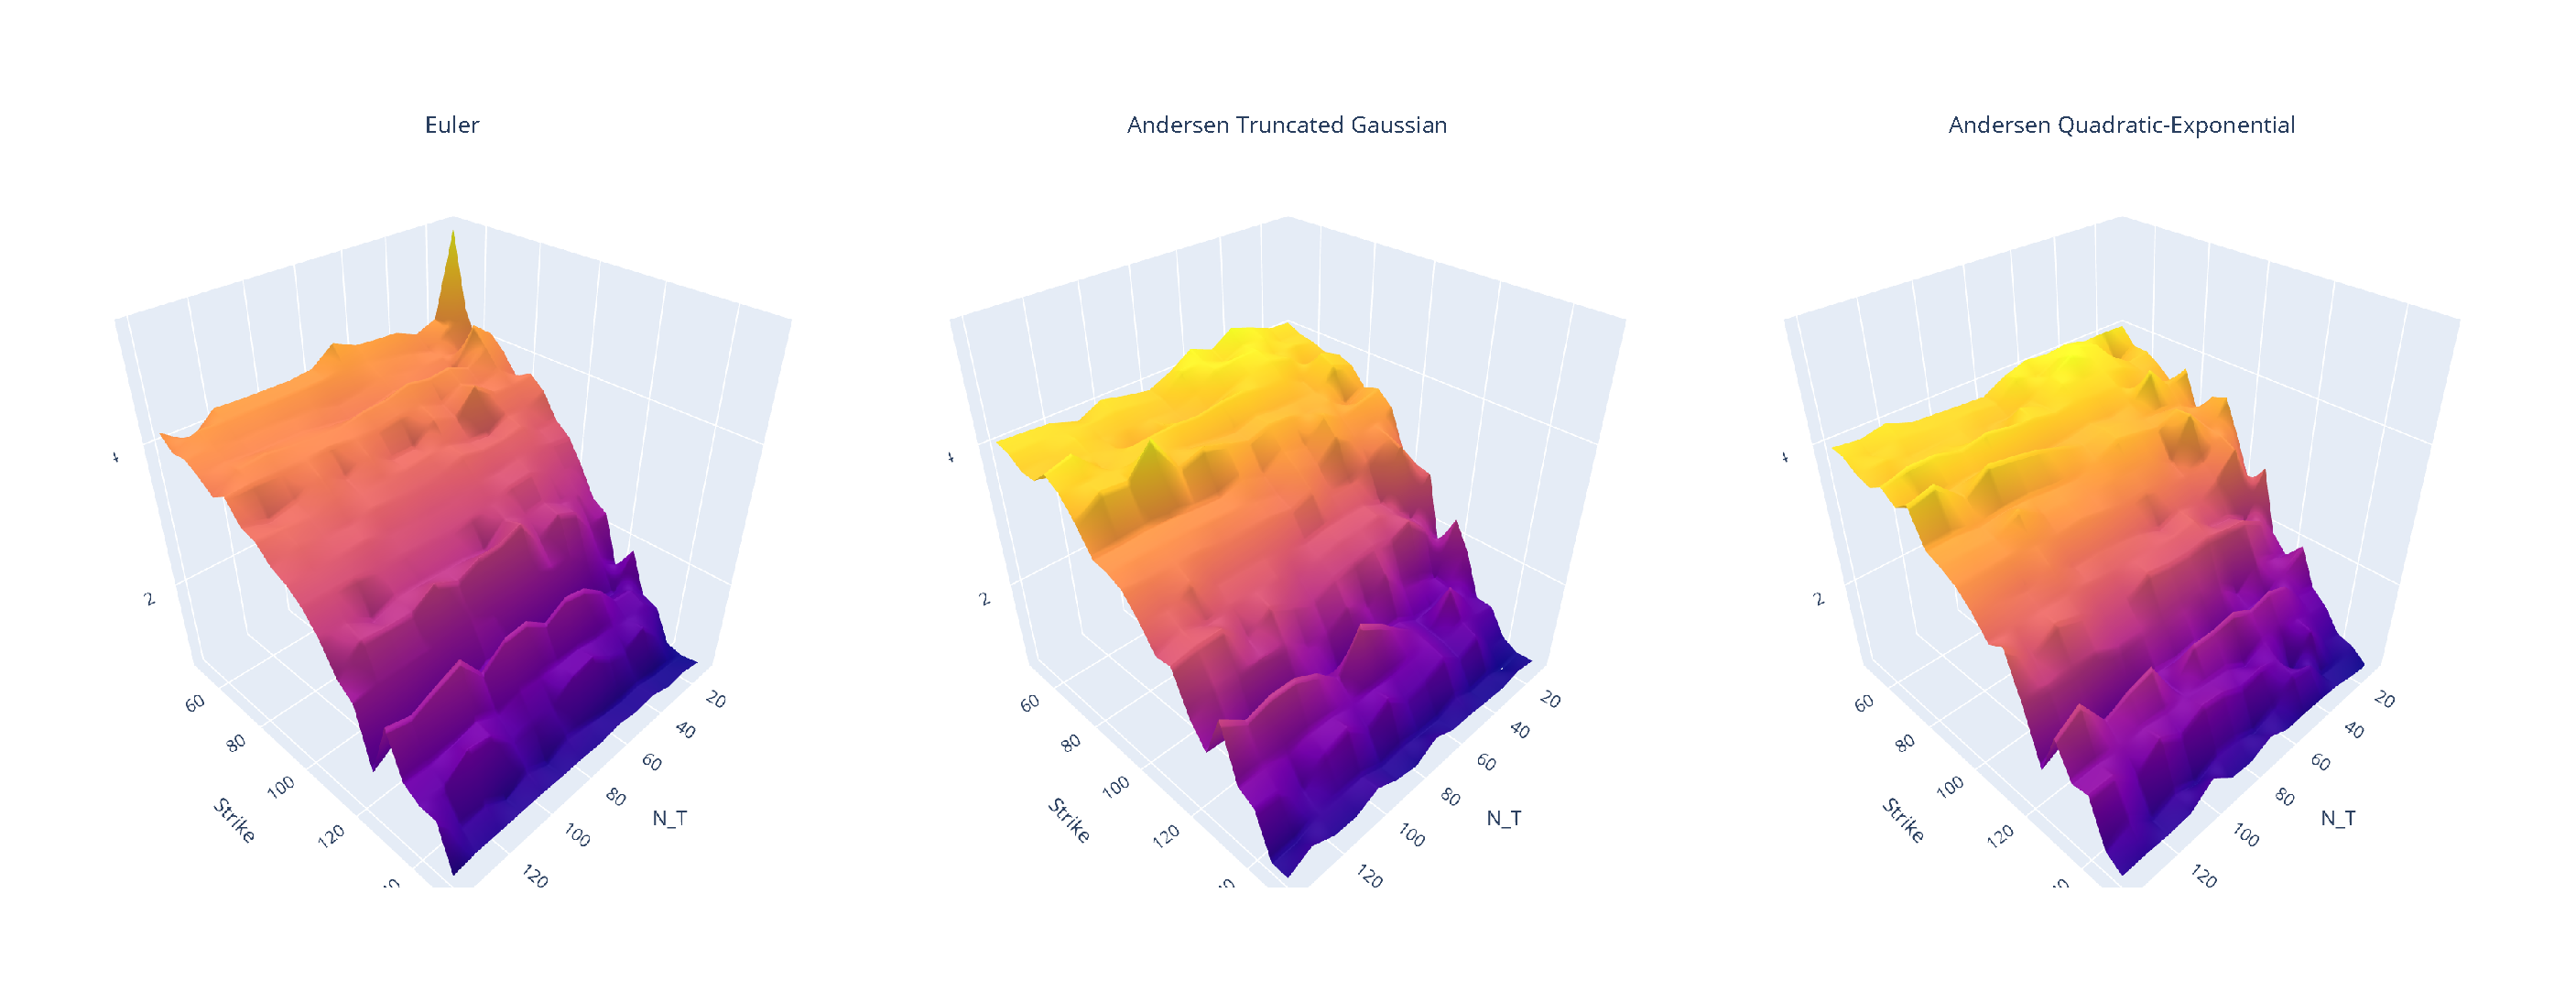
\includegraphics[width=\textwidth]{part5/pictures/surf_5.pdf}
        \end{figure}
    \end{frame}

    \begin{frame}{Control Variates}{Params \#5: $\kappa = 1$, $\gamma = 1$, $\rho = -0.3$, $\bar v = 0.04$, $v_0 = 0.09$, \texttt{absolute\_error = 5e-2}}
        \begin{figure}
            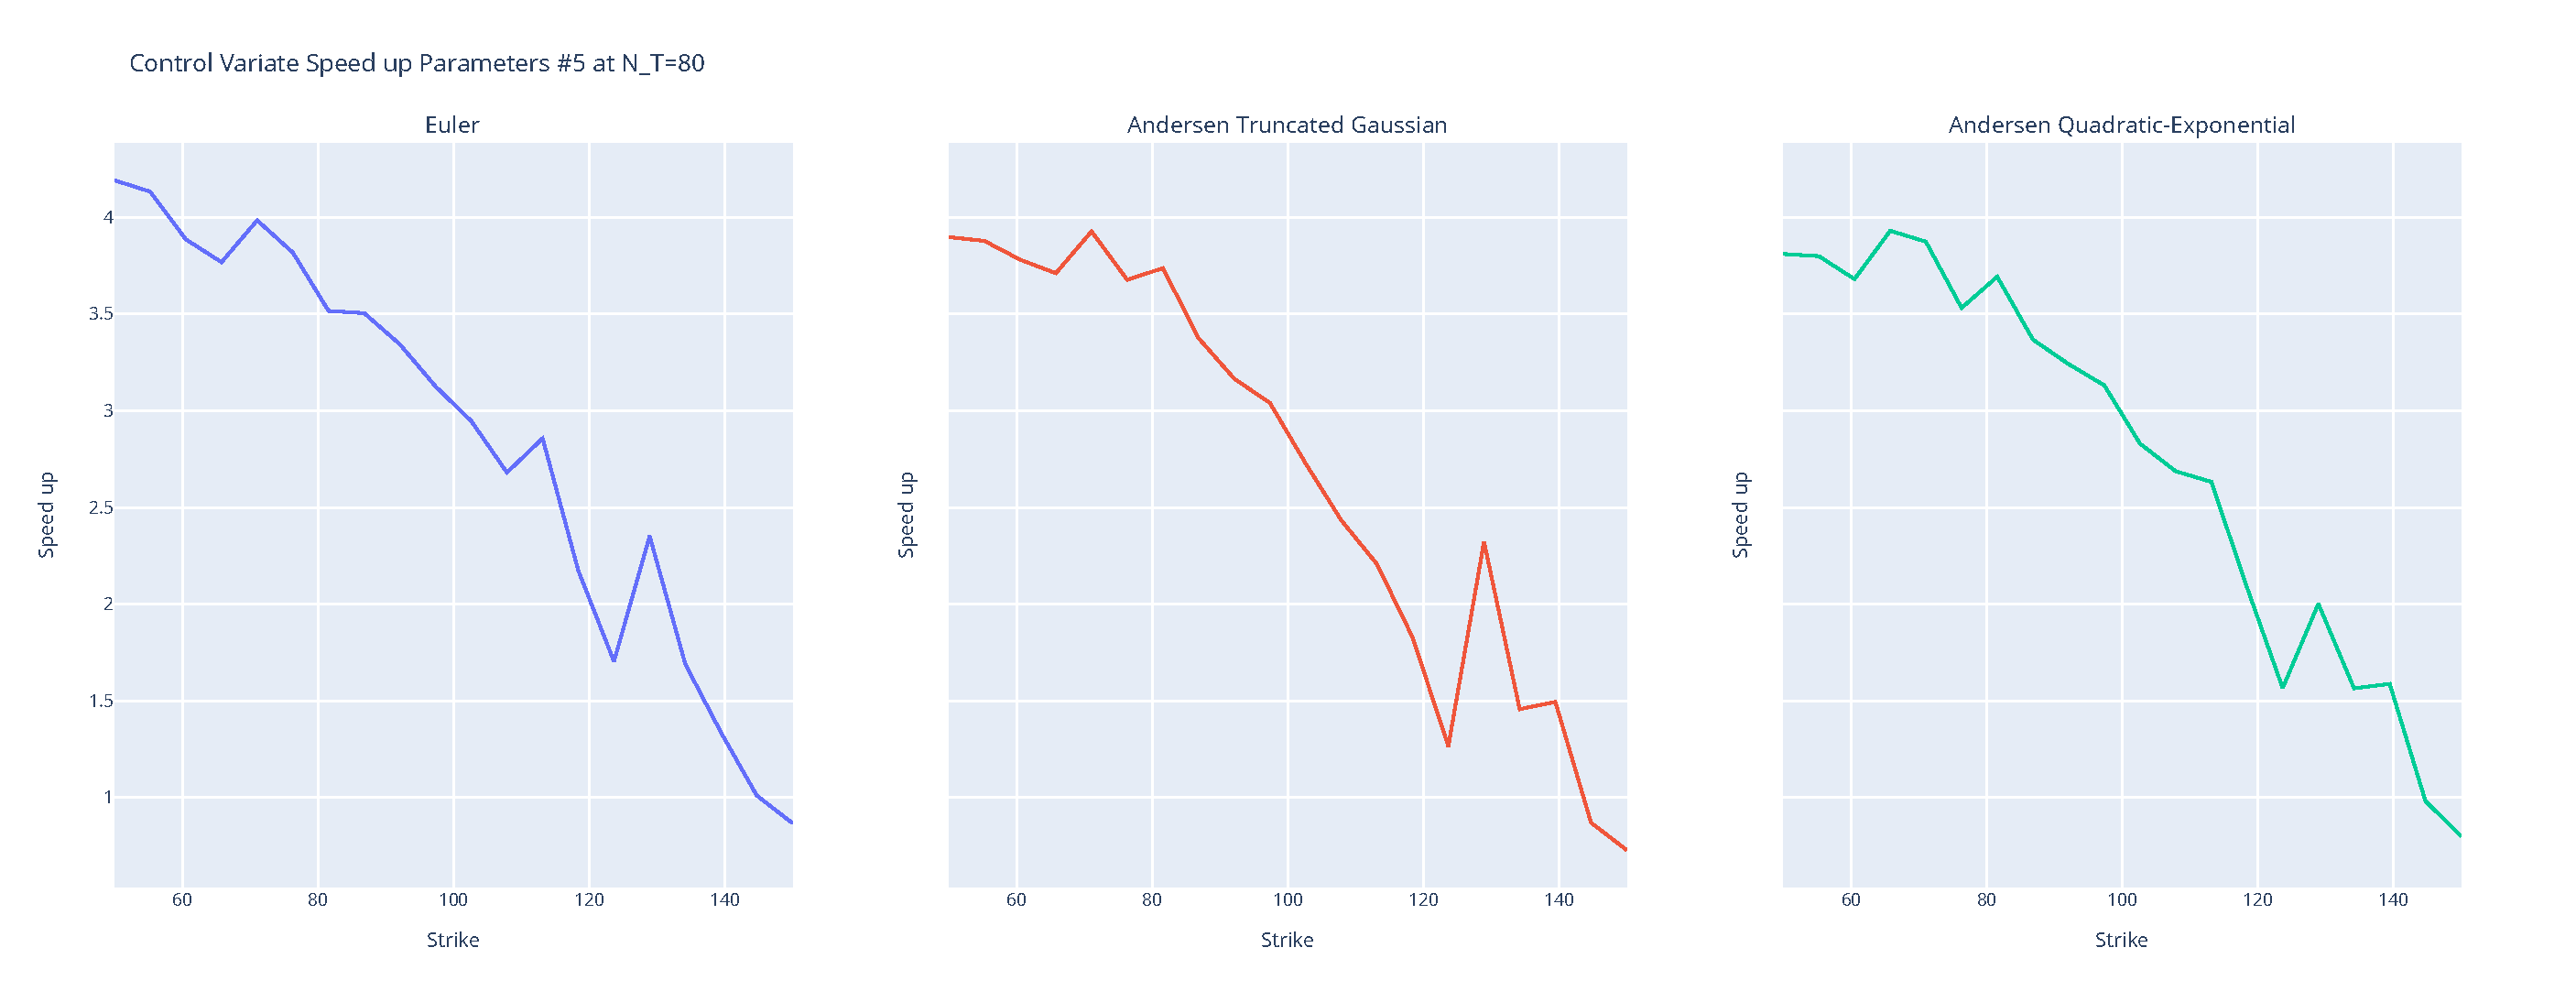
\includegraphics[width=\textwidth]{part5/pictures/pot_5.pdf}
        \end{figure}
    \end{frame}

    \begin{frame}{Antithetic Variates}{Params \#3: $\kappa = 0.5$, $\gamma = 1$, $\rho = -0.9$, $\bar v = 0.04$, $v_0 = 0.04$, \texttt{absolute\_error = 5e-2}}
        \begin{table}
            \begin{tabular}{lrrrrr}
                \toprule
                strike | T &     0.100 &     1.325 &     2.550 &     3.775 &     5.000 \\
                \midrule
                60.0   &  2.013505 &  2.207756 &  2.155487 &  2.208512 &  2.248140 \\
                80.0   &  1.849364 &  2.335388 &  2.062118 &  2.176501 &  2.133676 \\
                100.0  &  1.061477 &  1.625179 &  1.721840 &  1.900734 &  2.316427 \\
                120.0  &  0.732203 &  0.713929 &  0.743541 &  1.142146 &  2.173608 \\
                140.0  &  0.758740 &  0.713107 &  0.738851 &  0.727490 &  0.780455 \\
                \bottomrule
            \end{tabular}   
            \caption{Euler AV Estimator Speed-Up. N\_T = 50.}
        \end{table}         
    \end{frame}

    \begin{frame}{Antithetic Variates}{Params \#3: $\kappa = 0.5$, $\gamma = 1$, $\rho = -0.9$, $\bar v = 0.04$, $v_0 = 0.04$, \texttt{absolute\_error = 5e-2}}
        \begin{table}
            \begin{tabular}{lrrrrr}
                \toprule
                strike | T &     0.100 &     1.325 &     2.550 &     3.775 &     5.000 \\
                \midrule
                60.0   &  1.949344 &  1.756579 &  1.726879 &  1.688654 &  1.626986 \\
                80.0   &  1.704026 &  1.515961 &  1.673850 &  1.664354 &  1.678994 \\
                100.0  &  0.669384 &  1.123111 &  1.438825 &  1.512500 &  1.242045 \\
                120.0  &  0.692517 &  0.551672 &  0.617581 &  0.689563 &  0.864373 \\
                140.0  &  0.700559 &  0.587885 &  0.592445 &  0.525306 &  0.544784 \\
                \bottomrule
                \end{tabular}
            \caption{QE AV Estimator Speed-Up. N\_T = 50.}
        \end{table}         
    \end{frame}

    \begin{frame}{Antithetic Variates}{Params \#3: $\kappa = 0.5$, $\gamma = 1$, $\rho = -0.9$, $\bar v = 0.04$, $v_0 = 0.04$, \texttt{absolute\_error = 5e-2}}
        \begin{table}
            \begin{tabular}{lrrrrr}
                \toprule
                strike | T &     0.100 &     1.325 &     2.550 &     3.775 &     5.000 \\
                \midrule
                60.0   &  2.059236 &  2.250601 &  2.228231 &  2.505417 &  2.206968 \\
                80.0   &  1.838265 &  1.868023 &  1.998318 &  1.984901 &  2.155268 \\
                100.0  &  0.672273 &  1.201758 &  1.845470 &  1.818466 &  1.914416 \\
                120.0  &  0.741082 &  0.758342 &  0.720228 &  0.826217 &  1.090340 \\
                140.0  &  0.724028 &  0.707492 &  0.717789 &  0.730815 &  0.730584 \\
                \bottomrule
                \end{tabular}
            \caption{QE AV Estimator Speed-Up. N\_T = 50.}
        \end{table}         
    \end{frame}

    \section{Problems, Issues, and Plans}
        \begin{frame}{Conclusion}
            \begin{enumerate}
                \item We introduced the three common Heston simulation methods: Euler-Maruyama, Andersen TG and Andersen QE; 
                \item We compared the theoretical vanilla options prices and their Monte-Carlo counterparts;
                \item We measured the performance while pricing the exotics.
            \end{enumerate}
        \end{frame}
        
        \begin{frame}{To-dos}
            \begin{enumerate}
                \item Implement the Exact (Broadie and Kaya) scheme;
                \item Measure the presiceness of the pricers for the real market data;
                \item Part of the pricing library.
            \end{enumerate}
        \end{frame}

\end{document}
